\documentclass{report}
\usepackage[utf8]{inputenc}
\usepackage[T1]{fontenc}
\usepackage{longtable}
\usepackage{graphicx}
 \usepackage{array}
 \usepackage{caption}
 \usepackage{graphicx}
 \usepackage{rotating}
%\usepackage[italian]{babel}

%Disable all warnings issued by latex starting with "You have..."
\usepackage{silence}
\WarningFilter{latex}{You have requested package}
\pdfsuppresswarningpagegroup=1

%Bib
\usepackage[
backend=biber,
style=alphabetic,
sorting=ynt
]{biblatex}
\addbibresource{References.bib}

\usepackage{csquotes}
%\usepackage{natbib}


%Import

\usepackage{tabularx}
\usepackage{marvosym}
\usepackage{fancyvrb}
\usepackage[usenames]{color}
\usepackage[hidelinks]{hyperref}
\usepackage{url}
\usepackage{graphicx}
\usepackage{xcolor}
\usepackage{amsmath,amsfonts,amssymb,amsthm,mathtools}
\usepackage{caption}
\usepackage{enumerate}
\usepackage{multicol}
\usepackage{subcaption}
\usepackage{float}
\usepackage{indentfirst}
\usepackage{listings}
\usepackage{tocloft}
\usepackage[most]{tcolorbox}
\usepackage{pgfplots}
\usepackage{Style/pgfplotsthemetol}
\pgfplotsset{compat=1.16}
\definecolor{lstgrey}{rgb}{0.94,0.95,1}
\lstset{
    language=scala,
    backgroundcolor=\color{lstgrey},
    frame=single,
    rulecolor=\color{lstgrey}, % make frame "invisible"
    captionpos=t,
    tabsize=2,
    numberbychapter=false,
    showstringspaces=false,
    basicstyle=\footnotesize,
    breaklines=true,
}
%LINK CLICCABILI
\hypersetup{
    colorlinks = true,
    linkcolor = .,
    citecolor = {blue},
    linkbordercolor = {white},
    urlcolor = {blue},
}
%TABELLE TBCOLORBOX
\tcbset{
        enhanced,
        colback=red!5!white,
        boxrule=0.1pt,
        colframe=red!75!black,
        fonttitle=\bfseries
       }



%PATH IMMAGINI
\graphicspath{{Images/}{DrawIo/}}
\newcommand{\emailaddr}[1]{\href{mailto:#1}{\texttt{#1}}}

\title{\LARGE
    Smart DogHouse
}

\author{
    Kiade Sara \\ \emailaddr{sara.kiade@studio.unibo.it}
    \and 
    Caminati Gyordan \\ \emailaddr{gyordan.caminati@studio.unibo.it} 
    \and
    Lirussi Igor \\ \emailaddr{igor.lirussi@studio.unibo.it}
}

\date{\today}

\begin{document}
\maketitle
% -*- root: ../main.tex -*-
\begin{abstract}

\end{abstract}
\tableofcontents

% -*- root: ../main.tex -*-

% Esporre l'obiettivo del progetto dandone una visione complessiva. Devono essere illustrate le caratteristiche salienti del progetto; deve essere chiara la distinzione tra le tecnologie usate/assemblate durante lo svolgimento dell'elaborato e il contributo tecnologico/scientifico e effettivamente apportato dal gruppo.
% 3000 - 6000 battute

\chapter{Introduzione}
Smart DogHouse è un progetto che nasce con l'intento di migliorare le condizioni dei cani che si trovano ospiti di un \textbf{canile}, mediante l'introduzione di un \textbf{supporto informatico} che possa, da un lato, \textbf{facilitare operazioni} che già prima venivano svolte e dall'altro \textbf{introdurre nuovi strumenti} che vadano a migliorare la gestione del canile.

\section{Overview}
Come riferimento è stato preso in considerazione il \textbf{ canile comunale di Pisa}, il quale gestore si è offerto di indirizzarci permettendoci di rivolgerci a lui per avere feedback e indicazioni basate su \textbf{esperienze reali}. 

L'idea ha avuto origine dopo un colloquio con il gestore del canile che, raccontando la propria esperienza, ha evidenziato alcuni \textbf{problemi} che riscontra nello svolgimento del proprio lavoro, molti dei quali sono risolvibili attraverso gli \textbf{strumenti} e le \textbf{competenze} che abbiamo a disposizione.
Successivamente, le informazioni ottenute dal canile di Pisa sono state confrontate e integrate a fronte di un colloquio con il \textbf{canile Comunale di Cesena}, la quale consulenza è stata indispensabile per riuscire a discernere gli \textbf{aspetti comuni }alla maggior parte dei canili da quelle che invece sono \textbf{peculiarità} di un canile specifico. 
Le domande e le risposte di entrambi i canili sono rese disponibili nel \href{https://github.com/SmartDogHouse/Report/tree/main/Extra/Domande_Canile.pdf}{pdf relativo negli extra}.
Questa capacità di \textbf{astrazione} ci ha permesso di definire meglio gli \textbf{obiettivi}. 
Anche se questo non può essere considerato un progetto su commissione, abbiamo fede nel fatto che una volta sviluppata la nostra soluzione, essa possa essere utilizzata come base per sviluppare altri sistemi o rendere più tecnologici canili e gattili che riscontrano le stesse difficoltà.

        %CANILI
        \begin{figure}[H]
            \caption{I due canili interpellati in qualità di \textbf{esperti del dominio}}
            \label{fig:Canili}
            \centering
            
\includegraphics[width=0.8\textwidth]{Images/canili.png}
        \end{figure}

\section{Problemi}
Il canile di Pisa ospita circa una \textbf{sessantina} di cani e gatti di diversa \textbf{taglia}, \textbf{randagi} o \textbf{abbandonati}, che vengono prelevati dagli addetti del canile su segnalazione dei cittadini. I cani restano poi in cura finché non vengono \textbf{adottati}, mentre i gatti vengono \textbf{rilasciati} subito dopo aver ricevuto le cure  mediche ed essersi ripresi. Ad occuparsi della salute dei cani è un \textbf{responsabile sanitario} sempre presente nella struttura, che coordina alcuni \textbf{veterinari} convenzionati con la struttura. La situazione al canile di Cesena è similare, con la differenza che quest'ultimo non si occupa più del recupero di gatti randagi e il responsabile sanitario non coordina altri veterinari ma si occupa \textbf{in autonomia} di tutto ciò che riguarda la salute del cane, dai problemi di routine alle \textbf{operazioni chirurgiche}.

I principali problemi che vengono attualmente riscontrati sono i seguenti:
\begin{itemize}
    \item \textbf{responsabile sanitario:} il responsabile sanitario e alcuni veterinari convenzionati, risiedono all'interno del canile.
    Attualmente non è possibile monitorare in maniera continuativa lo stato di salute di un animale. Questo spesso si traduce in un intervento tardivo che porta con sé delle limitazioni che con una diagnosi più veloce si sarebbero potute evitare.
    \item \textbf{Rifornimento e consumi di cibo ed acqua:} in entrambi i canili la maggior parte del lavoro manuale viene svolta dai volontari che prestano attività in forma gratuita e fortemente discontinua. Non è possibile sapere a priori quanti volontari si presenteranno a dare una mano, ed essendo in tanti non è nemmeno possibile sapere chi ha svolto quali mansioni. Operazioni come il rifornimento di cibo ed acqua vanno quindi monitorate personalmente dal gestore che deve recarsi fisicamente nelle gabbie per controllare gli approvvigionamenti; inoltre non è nemmeno possibile conoscere la quantità di cibo ed acqua consumata da un cane, il che rende più difficile individuare i segnali alimentari che sono sintomi di alcuni problemi di salute.
    \item \textbf{Sorveglianza:} né il canile di Pisa, né quello di Cesena, attualmente, dispongono di un sistema di sorveglianza da remoto, pertanto nel momento in cui si verificano furti, effrazioni ed atti vandalici, non è possibile risalire agevolmente al colpevole. E' assente anche un sistema che possa permettere di sorvegliare da remoto cani che hanno particolari problemi. Nel caso di una gravidanza che volge al termine, ad esempio, il personale del canile è costretto a recarsi frequentemente sul luogo, durante la notte, per controllare se ha avuto inizio il travaglio o se si stanno verificando delle complicanze. Questa necessità crea un disagio al personale che si trova a doversi recare in canile fuori dall'orario di lavoro.
    
    \item \textbf{Assenza di supporto informatico}: attualmente nessuno dei due canili dispone di un'infrastruttura informatica già presente, da poter integrare; inoltre non dispongono nemmeno di un gestionale che dia supporto nella catalogazione degli animali presi in cura.
\end{itemize}
 




\section{Obiettivi}
L'obiettivo è quello di rendere il canile più "Smart", introducendo della strumentazione che permetta di risolvere in maniera parziale o totale le problematiche descritte precedentemente, mantenendo un costo accessibile. 

    \begin{figure}[H]
        \caption{Obbiettivi principali}
        \label{fig:Obbiettivi}
        \centering
       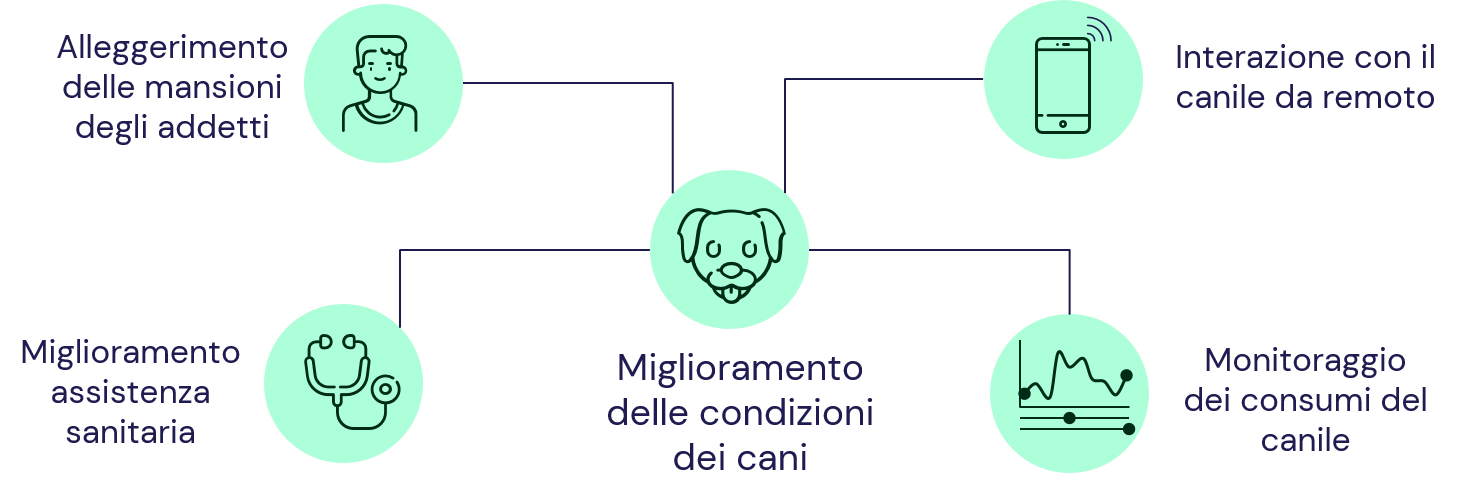
\includegraphics[width=1\textwidth]{Images/cani.png}
    \end{figure}
Nello specifico si vogliono incontrare le esigenze del gestore e degli addetti, agevolando le operazioni di:
\begin{itemize}
    \item \textbf{monitoraggio dello stato di salute dei cani} tramite:
    \begin{itemize}
        \item rilevazione dei \textbf{consumi} di cibo e acqua;
        \item monitoraggio del \textbf{comportamento} del cane.
    \end{itemize}
    In questo modo è possibile cogliere in maniera preventiva segnali che possono indicare un problema di salute e aiutare il \textbf{responsabile sanitario} nella risoluzione e nella diagnosi dello stesso. 
    \item automatizzazione delle operazioni di
\textbf{cura quotidiana} attraverso:
    \begin{itemize}
        \item automatizzazione del \textbf{rifornimento} di cibo e acqua
        \item possibilità di scegliere, per ciascun cane, la \textbf{quantità} del cibo da somministrare e la \textbf{frequenza}.
    \end{itemize}
    In questo modo è possibile gestire in maniera più precisa l'alimentazione dei cani e impostare delle quantità di cibo particolari in caso di condizioni di salute che richiedono un particolare piano alimentare, sollevando da questo incarico i volontari, che svolgono un'attività non tracciabile e discontinua. Inoltre, sarà possibile per il \textbf{responsabile sanitario} consultare i dati riguardanti l'alimentazione del cane e, di conseguenza, fornire diagnosi più precise. 
    \item \textbf{sorveglianza
globale del canile da remoto}: l'introduzione di un sistema di sorveglianza permetterà a chi di competenza di monitorare lo stato del canile anche da casa.
\item \textbf{Mantenimento dello storico dei dati registrati}: in questo modo sarà possibile consultare sia le informazioni riguardanti i cani che i dati che riguardano le condizioni del canile, permettendo anche di fare dei confronti su base temporale;
\item \textbf{consultazione dei dati acquisiti ed elaborati:} verrà fornita la possibilità di accedere allo storico dei dati medici su un Database, affinché il veterinario abbia una visione globale del quadro medico e possa velocemente filtrare le informazioni anche se non ha seguito il paziente dall'inizio. 
\item \emph{{[}optional{]}} 
\textbf{monitoraggio approfondito dei parametri vitali}: mediante l'installazione di sensoristica che permetta il monitoraggio di temperatura, battiti, movimento, ecc\ldots{} sarà possibile tenere ulteriormente sott'occhio cani che si trovano in condizioni di salute che necessitano di particolari attenzioni.

\item \textbf{Introduzione di un sistema informatico: } poiché non vi è un sistema informatico preesistente da integrare e vi sono poche disponibilità economiche, si è pensato di avvalersi di una piattaforma cloud sulla quale è possibile mantenere lo storico ed operare tramite l'utilizzo di un broker MQTT per la comunicazione  con sensori e attuatori. Questa soluzione è stata indicata come preferibile dal canile che ritiene più accessibile pagare mensilmente un servizio piuttosto che investire in una soluzione ad hoc. 

\end{itemize}






% -*- root: ../main.tex -*-
\chapter{Processo di Sviluppo}

\section{Domain Driven Design}
Il processo di sviluppo è stato guidato dalla filosofia data dal Domain Driven Design. La realizzazione di questo progetto costituisce, per i membri del team, un ottimo terreno di prova per mettere in campo molti degli aspetti di gestione propri di questo approccio.
    \subsection{Aspetti principali del DDD}
    Il Domain Driven Design è un approccio che si rivela ideale per la conduzione di progetti non banali che richiedono l'interazione di persone con background differenti. 
    L'obiettivo è quello di evitare gli errori comuni che tendono a verificarsi in mancanza di una buona gestione e comunicazione. Più che un pattern o un framework, il DDD è una filosofia che rappresenta una guida. 
    
    Il Domain Driven Design è un approccio operativo che tenta di uniformare il modello di dominio con l'artefatto generato, cercando di muovere concetti fondamentali per l'ambito all'interno del software e della documentazione, che dovranno quindi rispecchiare in dominio utilizzando il giusto linguaggio.
    Il classico approccio di standardizzazione delle pratiche di analisi e progettazione, tende a deviare il software lontano dal contesto di dominio. Questo rende il prodotto poco robusto e solo parzialmente coerente con l'ambito.
    Per questo il DDD non è vincolato ad una particolare tecnologia o pattern di design, favorendo lo sviluppo mirato caso per caso.
    Tenta di trasmettere i costanti cambiamenti del dominio nel prodotto mantenendo una dualità costante che consente di ottenere un prodotto più coerente e leggibile sia per il team che per il cliente. 
    
    Generalmente utilizzato per progetti sia di medie che di grandi dimensioni che evolvono nel tempo, non è una metodologia o un architettura. Può essere visto come un approccio che coinvolge più strati socio-tecnologici orizzontalmente, dal business ai vincoli implementativi fino alle buone pratiche di coding.
    
    
    
    Concetti chiave che DDD porta con sè:
    
        \begin{itemize}
        \item \textbf{Strategia}: ogni problema ha la sua soluzione, non esiste il famosa silver bullet, bisogna trovare il giusto approccio e non cercare di eccedere con eccessivi strumenti o tecniche ove non richiesti.
        Non tutte le parti del prodotto necessitano la stessa modellazione, applicare ogni feature dell' approccio DDD per tutti i problemi può portare a problemi peggiori.
        DDD impone di identificare e distinguere il \textbf{Core Domain}; la parte che detiene il business value maggiore e di dedicarvi più risorse e tempo.
        Mentre per le restanti parti, i \textbf{subdomain}, è possibile utilizzare un approccio più conservativo.
        
        \item \textbf{Learning}: forse il passo più critico per ottenere un prodotto di qualità. Il processo di apprendimento deve essere costante e continuativo, consentendo di diffondere un sapere condiviso che incentiva la comunicazione e agevola la costruzione di una soluzione coerente e coesa con la terminologia del dominio. 
        L'apprendimento ideale dovrebbe essere tale da faticare nel distinguere un \textbf{Domain expert} da un membro del team del progetto in chiave DDD.
        
        \item \textbf{Linguaggi}: la comunicazione è fondamentale all'interno di un team, il DDD spinge la classica comunicazione oltre i confini del team fino agli attori del dominio stesso promuovendo un linguaggio comune.
        Fondamentale che i concetti imparati e diffusi siano precisi, cercando di limitare o annullare l'ambiguità,tramite una serie raffinamenti che passa per il colloquio costante e la compartizzazione dei concetti.
        
        \item \textbf{Modelli multipli}: risolvere un problema con un singolo modello rende il tutto offuscato e poco strutturato, il DDD porta il concetto di \textbf{Divide et impera} a livello di modello promuovendo non solo una divisione il più semanticamente corretta e precisa ma anche una visione d'insieme fornita tramite una mappa delle interazioni che tenga traccia delle comunicazioni.
        Mette in campo anche pratiche per rendere il bordo dei concetti il più nitido e inalterato possibile.
        
        \item \textbf{Architetture sofisticate}: le tecnologie si sono evolute e il DDD ne ha preso nota, il DDD promuove l'utilizzo e la progettazione di architetture dedicate al problema e il distaccamento da approcci classici per le parti core del dominio.
        
        \item \textbf{Advance and clean coding}: il DDD non è adatto a progetti semplici one shot. Il suo focus risiede in quei prodotti fatti per evolversi e durare nel tempo, promuovendo lo studio continuo del dominio che è in costante cambiamento. Per questo non è sufficiente mantenere il codice alla buona. Al contrario è necessario mettere in campo tutte le good practice del caso, lasciando del clean code capibile e facilmente evolvibile in qualcosa anche di drasticamente diverso. 
        
        
    \end{itemize}
    
    
    
    Gli aspetti principali del DDD sono:
    \begin{itemize}
        \item \textbf{Dominio}: è l'area tematica in cui si inserisce il progetto che si vuole realizzare. La corretta definizione del dominio è di estrema importanza in quanto esso rappresenta il perno attorno a cui ruota tutto il DDD. La figura dell'esperto del dominio rappresenta pertanto una risorsa inestimabile poiché grazie ad essa è possibile avere una visione reale dell'ambiente in cui si andrà ad operare. 
        \item \textbf{Modello}: Una rappresentazione distillata delle regole, assunzioni e scelte del modello. Descrive e astrae dando una formula snella alle tematiche, utilizzato per risolvere problemi correlati al dominio stesso.
        \item \textbf{Ubiquitous language}: si tratta di un linguaggio condiviso tra sviluppatori, utenti e collaboratori, la quale definizione permette di facilitare la comunicazione tra persone con diversi background ed evitare ambiguità che portano a errori e incomprensioni.
        \item \textbf{Contesto}: %TODO
    \end{itemize}

\section{Metodologia di Sviluppo}
Per sviluppare il progetto è stata scelto il framework Scrum. Questo per permettere di mantenere alta la qualità e minimizzare il rischio nella produzione. Inoltre la sua natura iterativa e incrementale si presta bene allo sviluppo del progetto, di sua natura fortemente basato sull'interazione con il cliente. Tuttavia, essendo il team composto solo da 3 componenti, i quali lavorano sullo stesso progetto, ne è stata adottata una versione leggermente semplificata descritta in seguito. 
    \subsection{Scrum}
    Il processo di sviluppo Scrum-Inspired modifica in primis i ruoli: il committente è facilmente identificabile nel proprietario del canile, ma il product-owner e lo scrum-master sono sono essi stessi anche developer (parte del team di sviluppo). 
    Inoltre, particolare enfasi è stata posta sulla cross-fertilization, lo scambio di competenze, essendo il team piccolo ma molto eterogeneo, senza struttura interna.
    L'organizzazione delle attività è stata impostata attorno agli sprint, concetto chiave di Scrum. Ogni sprint fornisce una suddivisione temporale del progetto (composto sia dal software che dal report) definendo i meeting, gli obiettivi e i risultati perseguiti. Per ogni Sprint, seguendo il modello del framework, è stato definito un meeting iniziale di circa un'ora, di pianificazione. 
    Nello Sprint Planning, infatti, la divisione in due parti è stata unificata. Essendo il product-owner anche developer non può essere escluso dalla nella seconda parte come impone la metodologia Scrum. 
    All'interno del meeting iniziale dapprima le priorità degli item sono state assegnate da un membro del team, impersonando temporaneamente il product-owner. In seguito, è stato raffinato collaborativamente il product-backlog: gli item sono stati espansi e sono stati scelti sia i goals/obiettivi generali dello sprint corrente sia quali item prendere in carico per esso (unificando parte due dello Sprint Planning).
    Generato lo sprint-backlog, sottoinsieme del product-backlog, in cui sono presenti i task identificati in precedenza, questi vengono presi in base volontaria. 
    Ogni giorno, in seguito, è stato fatto il canonico daily-Scrum, per l'aggiornamento dei membri del team relativamente al potentially-shippable-product-increment dello sprint.
    Per identificare questo la "Definition of Done" è stata formalizzata collettivamente come: "il task è inteso completo se sono stati sviluppati, testati con successo e documentati".
    Infine è stato mantenuto il meeting finale, ma la suddivisione nelle tre parti anche qui è stata condensata. 
    Nel meeting la prima parte è stata dedicata al "refinement" del backlog, in cui si aggiorna in base a quello che è stato fatto. In seguito si è passati alla "sprint review" in cui si è condiviso con gli altri ciò che è stato fatto. Inoltre in questa fase è stato coinvolto il commitente, spesso per mezzo della piattaforma Telegram, per renderlo partecipe del progresso del progetto e verificare che questo proceda nella giusta direzione. In ultimo, nella "Sprint Retrospective", è stato discusso cosa ha funzionato e cosa no, quali aspetti organizzativi sistemare e correggere per il prossimo sprint. 
    
    
    
    

\section{Gestione di Progetto}
In questa sezione verrà spiegato come il progetto è stato organizzato dal punto di vista pragmatico, con quali strumenti e teconologie si è scelto di procedere.
    \paragraph{Gantt Chart}
    
    \paragraph{GitHub Projects Management}
    Per le Board di Scrum è stato utilizzato GitHub Projects. La scelta è ricaduta su questa opzione anziché sui competitor, quali Trello, data la possibilità di interazione con il progetto stesso e con le repository. 
    La struttura delle board è stata organizzata ad albero:
    Una board principale all'interno dell'organizzazione funge da Product-Backlog-Board. Questa viene mantenuta dal Product-Owner, egli sceglie per ogni Sprint la priorità degli Items. Questi vengono raffinati iterativamente, gli Item in cima infatti diverranno via via più specifici. Ad ogni sprint gli Item più importanti verranno inoltre eletti come Sprint Goals (COSA fare all'interno dello sprint). 
    Nel progetto gli item sono stati scelti in base alle User Stories e trasformati in Issue, da risolvere ad ogni sprint.
    All'interno delle repository invece sono stati incrementalmente implementate tante board quanti gli Sprint-Backlog. Questi tengono invece traccia degli specifici task da sviluppare all'interno dei singoli Sprint (COME raggiungere lo Sprint Goal) a partire dall/dagli Item selezionati. 
    Per il completamento dello Sprint Goal è stata presa in considerazione  la "Definition of Done" specificata in precedenza.
    Una board aggiuntiva è stata creata per tenere traccia dei progressi della relazione. Ogni capitolo è stato definito come milestone, completabile alla scrittura di tutti i sottocapitoli, identificati come task.
    I vari task sono stati divisi in categorie standard per lo Scrum: "to Do", "in Progress", "Done".
    
    \paragraph{Telegram}
    Come strumento di messaggistica informale all'interno del gruppo, si è scelta la piattaforma Telegram. Accessibile facilmente da smartphone e da computer permette di aggiornare i componenti del gruppo immediatamente qualora vi siano delle urgenze. Il punto di forza rimane la  possibilità di spedire file di tutti i formati e di poter inserire nel gruppo dei BOT per automatizzare alcune azioni, tra cui le notifiche. Un'overview più chiara dell'utilizzo dei BOT verrà fornita nella \autoref{chap:CI}.
    
    \paragraph{Discord}
    Discord, nota piattaforma di comunicazione VoIP, è stato utilizzato invece come strumento di comunicazione formale. Si è creato un server apposito per il progetto, chiamato "SmartDogHouseChannel", con multiple stanze lavoro per diverse occasioni.
    I canali vocali sono stati utilizzati anche per la condivisione dello schermo, fattore chiave per la sincronizzazione e la comprensione senza dispendio non necessario di tempo. 

\section{Continuous Integration e Automatizzazione}
\label{chap:CI}
In questo capitolo si analizza la parte di integrazione e automatizzazione sia del progetto software che della relazione. 
    \paragraph{Relazione di Progetto}
        Considerato che anche la Relazione deve essere versionata e automatizzata, essendo parte del software, abbiamo iniziato partendo da essa. 
        Come linguaggio di markup è stato scelto {\LaTeX}, per la sua flessibilità e potenza. 
        Come strumento per la compilazione invece è stato scelto Overleaf.com, poiché permette di collaborare sullo stesso progetto, in real-time, e di non dipendere da diversi IDE per {\LaTeX} installati in locale. 
        Overleaf inoltre è stato collegato al repo, permettendo di pushare i cambiamenti fatti in tutta fluidità. 
        Nel repository, tramite l'utilizzo di GitHub Actions, è stato implementato un processo di automatizzazione con multipli Job. 
        Il primo Job si attiva ad ogni push ricevuta, compila il Latex per mezzo di una action e, qualora si verificassero degli errori, li salva in un log più piccolo, che verrà caricato come artefatto. Invece, se nessun errore è presente, è il pdf generato a venire caricato come artefatto.
        La terminazione di questo Job attiva altri due Job, dipendenti, che si occupano delle notifiche Telegram. Anche qui per mezzo di una action viene mandato un messaggio di notifica sul gruppo, sia se la build del Latex ha avuto successo, sia che ci siano stati errori. In caso di fallimento assime al messaggio viene inoltrato sul gruppo pure il log conciso che contiene solo gli errori Latex. 
        Per la gestione delle release è stato inoltre implementato un altro Job che verifica se nel messaggio di commit è presente uno speciale segnalatore -TAG{}. 
        La scelta di gestire la numerazione dei tag a mano è stata dettata dalla necessità di controllo e cusotomizzazione di questi: in una relazione si vuole scegliere quando effettuare la release e, adottando il semantic versioning, il grado di cambiamento che si ritiene più opportuno.
        Il Job successivo si occupa del deploy, e viene attivato solamente se è stato trovato un tag nella parte precedente. Questo Job scarica il pdf precedentemente generato negli artefatti e si occupa di farne una release con nome coerente e con il tag specificato. 
        Al termine della release vengono lanciati altri due Job, anch'essi dipendenti, che si occupano di notificarne il completamento. 
        Il primo usa una GitHub Action per inoltrare una mail ai componenti del gruppo contenente il pdf della release. Per fare ciò si è dovuto creare un account Gmail specifico che funge da casella di invio. Si può inoltre sfruttare come account di notifica per un'eventuale newsletter agli iscritti ad ogni nuova release. 
        Il secondo Job si occupa parallelamente di inoltrare un messaggio Telegram sul gruppo dei developers contentente anch'esso il pdf della release, il responsabile e il testo del commit.
        Un ultimo Job è stato creato per gestire anche le GitHub Pages, le quali forniscono un sito in cui consultare la relazione online. Per fare ciò è stato   creato un nuovo branch sul quale viene fatto il commit dei file Html generati grazie a Pandoc.
        \begin{figure}[h]
            \caption{Pipeline implementata, esecuzione di un commit senza tag}
            \centering
            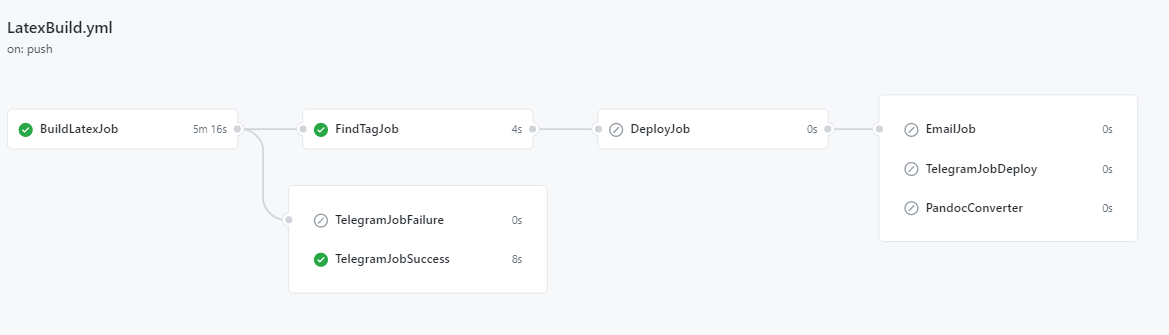
\includegraphics[width=1\textwidth]{RepoCI.png}
        \end{figure}
        
        \subparagraph{Tool utilizzati}
        \begin{itemize}
            \item Overleaf
            \item Draw.io
            \item GitHub Actions
            \item Telegram Bots
            \item Pandoc
            \item GitHub Pages
        \end{itemize}

    \paragraph{Progetto}
        
        \subparagraph{Tool utilizzati}
        GitHub Actions
        Telegram Bots
        Dependabot
        Test/Coverage









% -*- root: ../main.tex -*-
\chapter{Analisi dello spazio del problema}

	\section{Knowledge crunching}
	Seguendo le prime fasi del DDD, per carpire i concetti più fondamentali, sono stati interpellati gli esperti del dominio per via telematica. 
	Inizialmente è stata fatta una grande sessione collaborativa di Knowlege Krunching, per portare il team da 0 a una conoscenza adeguata del dominio e colmare le carenze di conoscenze dell'ambito del team di sviluppo. Questo è orientato a creare un grado di comprensione idonea del problema a permettere il kick-off del progetto.  
	Successivamente il processo è stato continuo, gli incontri sono stati periodici, per controllare che l'andamento del progetto proseguisse nella direzione sperata e per capire che alcuni concetti chiave non fossero sottovalutati o non compresi. 
	Per motivi di chiarezza riassumiamo tutto il processo nel seguente capitolo.
	Data l'ovvia problematicità nell'incontrarsi, è stata utilizzata la piattaforma di messaggistica Telegram (per chiamate vocali e brevi chiarimenti) e Discord (per la condivisione schermo con gli artefatti visuali). Durante le interazioni sono stati creati multiple rappresentazioni visuali a guida e supporto della conversazione. 
	Il gruppo parlando con il responsabile del canile (il maggiore esperto del dominio) ha indagato con maggiore enfasi i concetti necessari per la creazione di un buon software, tralasciando dettagli pleonastici. Il focus è stato su capire quello che serve per creare un software che soddisfi le reali necessità del cliente. I dettagli su cui l'esperto del dominio ricadeva spesso, infatti, hanno rivelato dove le energie dovessero essere maggiormente spese. 
	In questo caso gli esperti del dominio sono anche i clienti. Questi ultimi forniscono il problem-space, mentre i primi forniscono il solution-space.
	
	Per la comprensione degli obbiettivi di più alto business value, si è costruita in maniera interattiva e collaborativa un impact map, sotto la supervisione di team, scrum master e product-owner. Per non sfociare in un diagramma troppo informale.
	%IMPACT MAP DIAGRAM
	\begin{figure}[ht]
        \caption{Impact-map obbiettivi buiseness}
        \centering
        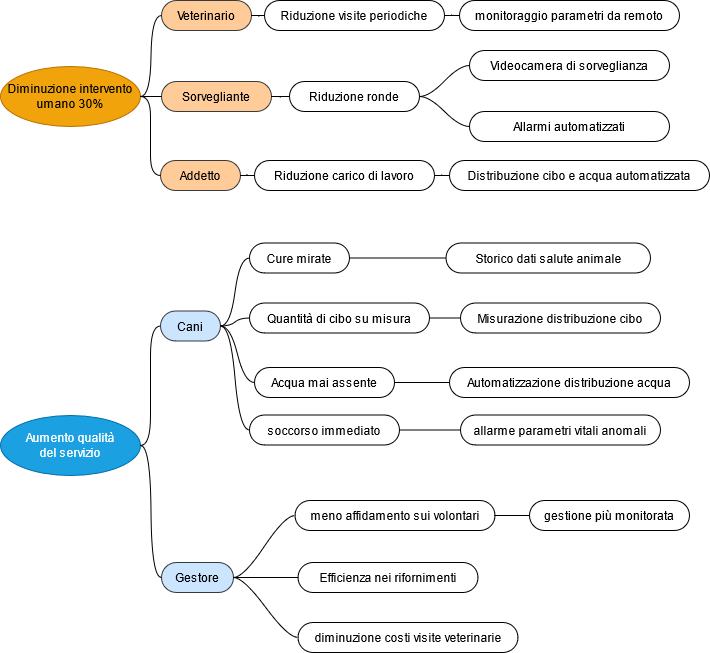
\includegraphics[width=1\textwidth]{DrawIo/impactMap.png}
    \end{figure}

    Il risultato ha portato in evidenza i due principali obbiettivi di business, evidenziando in maniera chiara la loro suddivisione, e le relative operazioni per raggiungere i risultati attesi.
    
    Con una visone d'insieme leggermente più definita, ci siamo cimentati nella stesura delle \textbf{user stories}. Cercando di seguire i due requisiti di business individuati, sono state identificate le più calzanti user stories per ogni obiettivo  dell'\textbf{impact map}
    .
    Nel tentativo di formalizzare le informazioni ottenute abbiamo suddiviso, raccolto e identificato le principali entità presenti. Sono state utilizzate successivamente per la definizione degli \textbf{use case diagram} che ne descrivessero le operazioni fondamentali.

	La definizione delle user-stories ha portato naturalmente a indagare il significato di alcuni termini usati. Questo ha spinto subito allo sviluppo di un ubiquitous language per i vocaboli più importanti, che poi è stato continuamente raffinato durante i successivi meeting. 
	Nel prossimo capitolo viene analizzato questo processo. 
    
	\section{Definizione Ubiquitus language}	
	L'Ubiquitous Language deve essere espresso nel modello di dominio, infatti unisce le persone del team di progetto.
    Lo scopo è eliminare le imprecisioni e le contraddizioni degli esperti di dominio, non è infatti imposto da questi, ma raggiunto collaborativamente.
    L'Ubiquitous Language si evolve nel tempo, non è definito interamente in una sola riunione, i concetti spesso si aggiungono, vengono sviscerati e partecipano nella comprensione del dominio. Infatti quelli che non fanno parte dell'Ubiquitous Language devono essere rifiutati.
    
    %TABELLA UBIQUITOUS LANGUAGE
    \begin{figure}[ht]
        \caption{Tabella ubiquitous language}
        \centering
        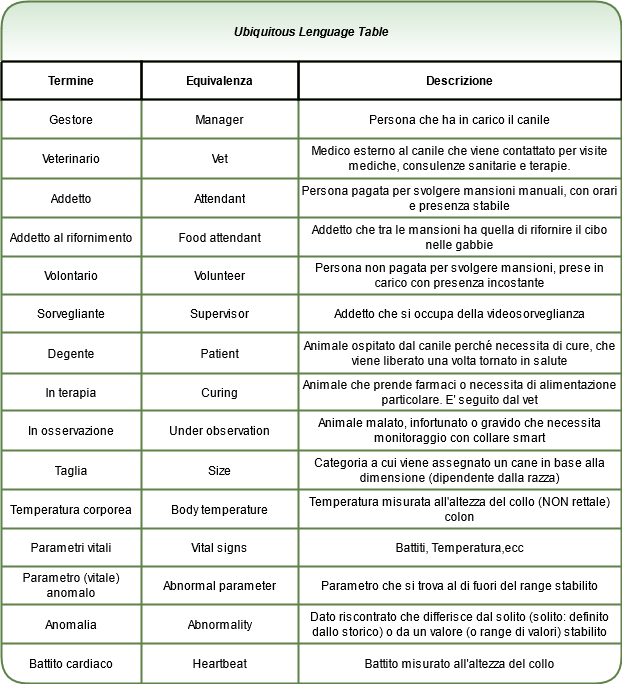
\includegraphics[width=1\textwidth]{DrawIo/ubiquitousLanguage.png}
    \end{figure}


\chapter{Analisi dei Requisiti}
In questa fase sono stati individuati i \textbf{requisiti del sistema}, partendo dalle descrizioni di alto livello, ottenute dal committente durante il \textbf{knowledge crunching}. Successivamente si è proceduto con un raffinamento che ha portato alla definizione di requisiti più \textbf{specifici}, \textbf{chiari} e \textbf{strutturati}.
	\section{Requisiti di Business}
	Si definiscono di seguito le aspettative del cliente e i requisiti che il prodotto dovrà soddisfare, espressi con una terminologia ad elevato livello astrattivo.
        \begin{itemize}
            \item Il prodotto dovrà \textbf{diminuire l'intervento umano} necessario per la quotidiana cura degli ospiti (Riempimento ciotola acqua/cibo); la riduzione del lavoro deve essere maggiore o uguale al 30\%.
            \item Il prodotto dovrà consentire di \textbf{diminuire il lavoro su base volontaria}, grazie alla riduzione delle operazioni di cura quotidiana, permettendo ai volontari di concentrarsi solo sulla socializzazione e lo svago dell'animale.
            Diminuisce così l'interferenza al di fuori delle loro mansioni, e migliora la tracciabilità del lavoro svolto, essendo il lavoro volontario incostante e meno affidabile.
            \item Opzionalmente il prodotto dovrà \textbf{fornire un monitoraggio a distanza} degli animali ospitati.
            Questo consentirà al personale incaricato di monitorare parametri come: frequenza cardiaca e temperatura corporea. Verrà diminuito anche l'intervento veterinario, non essendo necessaria la presenza in loco del professionista. La riduzione delle presenze dovrà consentire di diminuire i costi di un valore maggiore o uguale al 10\%.
        \end{itemize}
	
	\section{Requisiti Utente}
	Di seguito vengono riportate le richieste mosse dal cliente in maniera informale evitando termini tecnici, successivamente tali richieste saranno formalizzate per quanto possibile.
	Il prodotto dovrà fornire: 
		\begin{itemize}
            \item l'accesso al sistema da qualunque dispositivo munito di connessione alla rete, anche esterna al canile
            \item prestazioni adeguate alle operazioni richieste (con soglie adeguate caso per caso), come il rilevare se il cane ha bisogno di cibo o acqua 
            \item una restrizione delle funzionalità disponibili in base all'utente
            \item un interfaccia intuitiva, comprensiva di una pagina per l'accesso e un menu principale
            \item uno storico per ogni animale
            \item un accesso rapido e reattivo evitando tempi troppo lunghi per le operazioni
            \item un sistema di sorveglianza semi automatizzato in grado di identificare eventuali anomalie, come cani che escono senza permesso
            \item \textbf{opzionalmente} delle notifiche sullo stato di salute dell'animale al personale
            \item delle notifiche in caso di malfunzionamento del sistema stesso
            \item delle notifiche, nel caso in cui il cibo sia in esaurimento 
        \end{itemize}
        \subsection{User stories}
        Di seguito sono riportate tutte le \textbf{user stories} ritenute utili per lo sviluppo del prodotto.
        \begin{itemize}
            \item Come \textbf{gestore}
            voglio:
            \begin{itemize}
                \item poter visualizzare le i dati relativi all’occupante di una gabbia
                \item voglio poter impostare i dati dell’occupante di una gabbia
                \item poter rimuovere un cane da una gabbia
                \item poter visualizzare i consumi TOTALI del canile
                \item \textit{opzionalmente} poter visualizzare l’umidità e la temperatura ambientale 
                \item poter \textbf{impostare} i dati relativi allo \textbf{stato di salute} di un cane
                \item poter visualizzare i \textbf{consumi di cibo} relativi a un cane in un determinato lasso di tempo
                \item poter visualizzare i \textbf{consumi di acqua} relativi a un cane in un determinato lasso di tempo
            \end{itemize}
            
            \item Come \textbf{responsabile sanitario}
            voglio:
            \begin{itemize}
                \item \textit{opzionalmente} poter \textbf{visualizzare i battiti} di un cane 
                \item  \textit{opzionalmente} ricevere una \textbf{notifica} in caso di rilevazione di \textbf{anomalie} nei \textbf{battiti} o nella di un cane
                \item \textit{opzionalmente} poter \textbf{visualizzare la temperatura corporea} di un cane
                \item \textit{opzionalmente} ricevere una \textbf{notifica} in caso di rilevazione di \textbf{anomalie} nella \textbf{temperatura} corporea di un cane
                 \item \textit{opzionalmente} poter \textbf{impostare} gli intervalli di \textbf{temperatura e battiti} fuori dai quali vi è un’anomalia
                \item poter \textbf{impostare} gli intervalli delle \textbf{quantità di cibo e acqua } assunti, fuori dai quali vi è un’anomalia
                \item ricevere una \textbf{notifica} in caso di \textbf{anomalie} nella quantità di \textbf{acqua} assunta da un cane
                \item ricevere una \textbf{notifica} in caso di \textbf{anomalie} nella quantità di \textbf{cibo} assunto da un cane
                \item poter \textbf{impostare} i dati relativi allo \textbf{stato di salute} di un cane
                \item poter \textbf{impostare la quantità di cibo} da erogare a un cane
                \item poter visualizzare i \textbf{consumi di cibo} relativi a un cane in un determinato lasso di tempo
                \item poter visualizzare i \textbf{consumi di acqua} relativi a un cane in un determinato lasso di tempo
            \end{itemize}
            
            \item Come \textbf{addetto ai  rifornimenti}
            voglio:
            \begin{itemize}
                \item che la distribuzione di cibo agli animali sia automatizzata
                \item che la distribuzione di acqua agli animali sia automatizzata
                \item essere notificato se in una gabbia sta per esaurirsi il cibo
                \item ricevere una notifica in caso di malfunzionamento al sistema
                \item poter impostare la quantità di cibo da erogare a tutti i cani di una determinata taglia
                \item poter \textbf{impostare la quantità di cibo} da erogare a un cane
                \item poter visualizzare i \textbf{consumi di cibo} relativi a un cane in un determinato lasso di tempo
                \item poter visualizzare i \textbf{consumi di acqua} relativi a un cane in un determinato lasso di tempo
            \end{itemize}
            
            \item Come \textbf{addetto alla sorveglianza}
            voglio:
            \begin{itemize}
                \item poter visualizzare le immagini acquisite dalla videocamera di sorveglianza
                \item notificato in caso di uscita non autorizzata di un cane
                \item \textit{opzionalmente} essere notificato in caso di rilevazione di suoni forti o anomali
                \item \textit{opzionalmente} poter visualizzare l’umidità e la temperatura ambientale 
            \end{itemize}
        \end{itemize}
        
        Di seguito viene riportato lo schema, sotto-forma di diagramma di Venn, esplicativo delle intersezioni tra le User-Stories e le figure dell'organigramma. 
        %TABELLA CONTEXT MAP
        \begin{figure}[ht]
            \caption{Diagramma di Venn delle User-Stories}
            \centering
            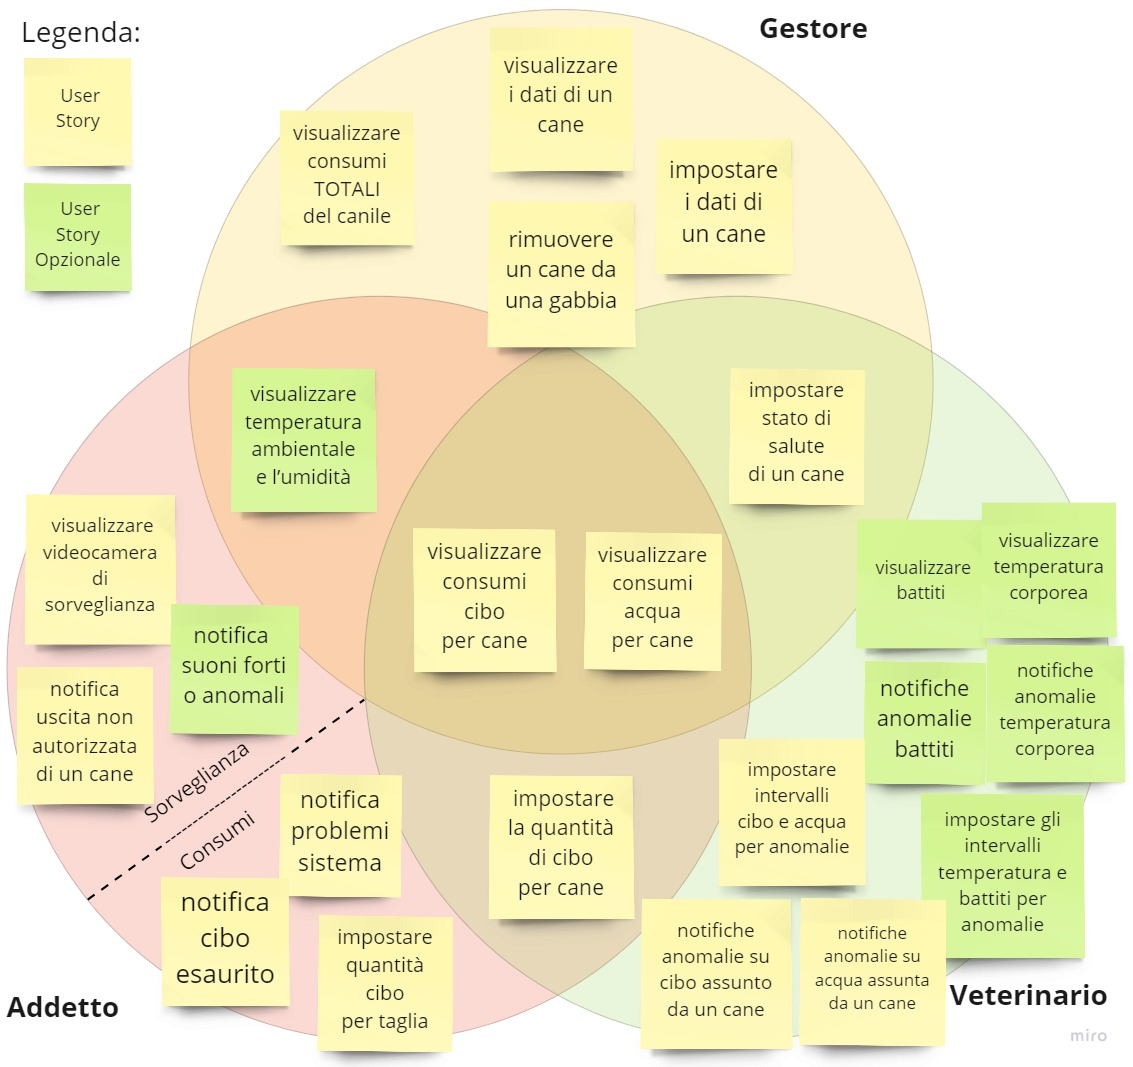
\includegraphics[width=1\textwidth]{Miro/DiagrammaUserStories.jpg}
        \end{figure}
    
	    
	\section{Requisiti Funzionali} %obbligatori, desiderabili e opzionali
	    \subsection{Casi d'uso}
        	 %Diagramma dei casi d'uso
            \begin{figure}[H]
                \caption{Diagramma dei casi d'uso del sistema, rappresenta le principali azioni effettuate degli attori}
                \centering
               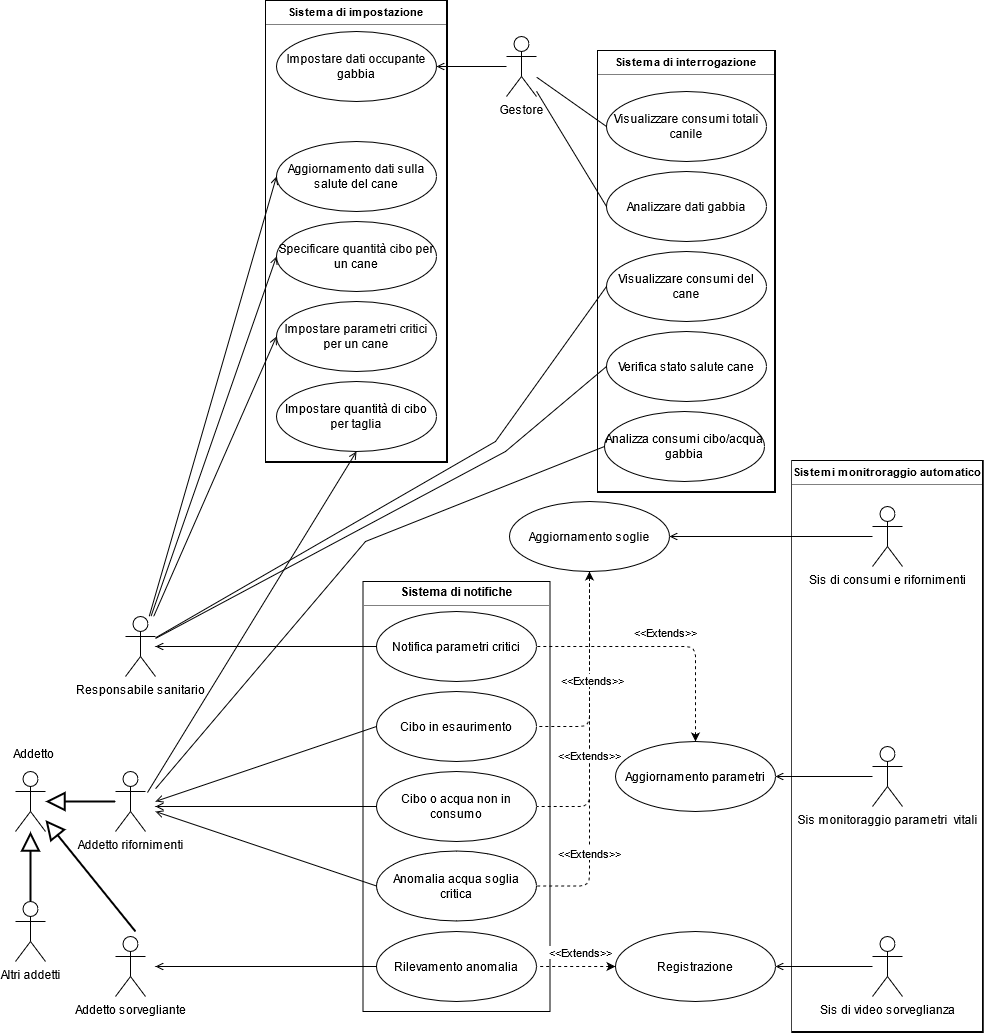
\includegraphics[width=0.9\textwidth]{DrawIo/useCaseWholeSystem.png}
            \end{figure}
            
    	Si elencano i requisiti funzionali per ognuno dei seguenti macro-componenti:
	    \begin{itemize}
            \item Applicativo web 
            \item Opzionale collare
            \item Strumentazione gabbia
            \item Strumentazione videosorveglianza
        \end{itemize}
        
    \subsection{Applicativo web}
        L'applicativo web deve consentire ad ogni utente di accedere con una serie di credenziali, e dividere le operazioni consentite in base ai permessi concessi.
        Il sito è suddiviso in tre pagine principali:
        \begin{itemize}
            \item \textbf{pagina di login}
                La pagina iniziale a cui ogni utente deve far riferimento per effettuare l'accesso.
                Sostanzialmente contiene solo gli elementi necessari per effettuare il \textbf{login}, non è prevista una funzione di registrazione autonoma.
            \item \textbf{home gestore}
                Il gestore ha accesso alla pagina di amministrazione, dov'è possibile:
                \begin{itemize}
                    \item registrare un nuovo utente
                    \item eliminare un utente
                    \item visualizzare le statistiche del canile
                \end{itemize}
            \item \textbf{home addetto rifornimenti}
                La schermata deve consentire di:
               \begin{itemize}
                    \item visualizzare le eventuali notifiche
                    \item visualizzare i consumi di un cane
                    \item impostare la quantità di cibo adeguata per taglia di cane
                \end{itemize}
            \item \textbf{home addetto sorveglianza}
                La home del sorvegliante deve fornire:
               \begin{itemize}
                    \item un accesso in diretta alle videocamere disponibili
                    \item deve essere possibile aggiungere o rimuovere una videocamera
                    \item visualizzare le notifiche se presenti
                \end{itemize}
            \item \textbf{home altri addetti}
                In un futuro sviluppo del prodotto è certamente contemplata l'aggiunta di altre mansioni o addetti.
            \item \textbf{responsabile sanitario}
                La pagina deve consentire di:
               \begin{itemize}
                    \item visualizzare lo stato di salute di un cane
                    \item visualizzare i consumi di un cane
                    \item impostare la quantità di cibo per un cane degente o in terapia
                    \item aggiornare lo stato di salute di un cane
                \end{itemize}
        \end{itemize}
        
    Nonostante un addetto possa ricoprire più ruoli, è stato scelto di modellare separatamente ogni mansione, questo consente: un maggiore controllo, rende più chiara la struttura e aiuta il lettore nella comprensione.
    Inoltre l'applicativo consentirà ad un utente di detenere uno o più ruoli, rendendo più agevole l'utilizzo. 
    \subsection{Opzionale: collare}
        Il collare smart deve costantemente inviare aggiornamenti sui parametri vitali dell'animale quali:
            \begin{itemize}
                \item La frequenza cardiaca
                \item La temperatura dell'animale
            \end{itemize}
    \subsection{Strumentazione gabbia}
        La gabbia smart deve:
            \begin{itemize}
                \item monitorare il consumo di cibo e acqua del cane inviando aggiornamenti costanti
                \item rifornire la ciotola di acqua quando troppo bassa
                \item rifornire la ciotola di cibo con la quantità desiderata quando
                mancante
                \item notificare la mancanza di cibo nel serbatoio
            \end{itemize}
    \subsection{Strumentazione videosorveglianza}
        La strumentazione deve fornire uno streaming video e audio costante nel tempo. La bidirezionalità è opzionale.
        
	\section{Requisiti non Funzionali}
	Il primo vicolo individuato è quello economico. Il costo del servizio, essendo l'attività non a scopo di lucro e mantenuta grazie all'azione dei volontari, deve essere minimo. Questo è comprensivo dell'istallazione, dei materiali e dei costi di servizio.
	Un secondo vincolo rappresenta la sicurezza, l'eventuale introduzione di strumentazione all'interno del canile non deve rappresentare in alcun modo un pericolo per la salute dell'animale.
	
    Il sistema dovrà rispettare alcuni requisiti non funzionali che ne determineranno la \textbf{qualità}:
        \subsection{Di Sistema}
            \begin{itemize}
            \item \textbf{Reattività}: 
            \begin{itemize}
                \item l'utente non deve percepire \textbf{ritardi} nell'ordine dei secondi tra l'invio di un comando e l'esecuzione dello stesso all'interno della piattaforma. 
                \item le notifiche standard del sistema devono essere mostrate ai relativi utenti con un ritardo complessivo massimo non superiore al minuto.
                \item le notifiche urgenti del sistema, ossia quelle relative a malfunzionamenti gravi o alla salute dell'animale, devono essere mostrate ai relativi utenti con un ritardo complessivo massimo non superiore ai dieci secondi.
            \end{itemize}
            
            \item \textbf{Scalabilità}: L'applicativo deve necessariamente consentire di aumentare o diminuire il numero di animali gestiti. Ciò deve avvenire senza una sensibile ripercussione sulle prestazioni del sistema e un disagio minimo a livello pratico. Per prevenire, inoltre, che la presenza di una connessione cablata limiti la scalabilità del sistema, è desiderabile che non ci siano altri collegamenti al di fuori dell'alimentazione già presente. 
            
            \item \textbf{Fault tolerance}: la \textbf{gestione degli errori} deve essere adeguatamente implementata affinché le interruzioni involontarie non danneggino innanzitutto la salute degli animali.
            Eventuali malfunzionamenti di apparecchiature o sensoristica all'interno del canile non devono pregiudicare il funzionamento complessivo dell'applicativo, ma al massimo della singola unità logica. 
    \end{itemize}
        
    \subsection{Della Sensoristica}
    \begin{itemize}
        \item \textbf{Precisione}:
            \begin{itemize}
                \item \textbf{Bilancia} lo scostamento massimo tra più misure deve essere inferiore o uguale a 10 grammi.
                \item \textbf{Temperatura} lo scostamento massimo tra più misure deve essere inferiore o uguale a 2 gradi.
                \item \textbf{Umidità} lo scostamento massimo tra più misure deve essere inferiore o uguale a 5\%.
                \item \textbf{Livello acqua} lo scostamento massimo tra più misure deve essere inferiore o uguale a 1 centimetro.
                \item \textbf{Frequenza cardiaca} lo scarto tra misure sulla stessa frequenza deve essere al massimo 10 battiti.
            \end{itemize}
        \item \textbf{Risoluzione}:
            \begin{itemize}
                \item \textbf{Bilancia} il range di misura, partendo da vuota, deve riuscire a comprendere almeno un Kg.
                \item \textbf{Temperatura} il range deve variare tra 0 e 50 gradi. %considerato che i cani piccoli crepano a -6 e i grandi a -12, ma tanto a 0 gradi sono tutti in temperatura critica direi che ci sta
                \item \textbf{Umidità} il range di umidità deve essere incluso tra 20-80\%.
                \item \textbf{Livello acqua} Il range deve variare almeno di tre cm. 
                \item \textbf{Videocamera}: necessaria almeno una risoluzione di 420p, non è richiesta la visione notturna. 
                \item \textbf{Frequenza cardiaca} la misurazione deve essere in grado di rilevare una frequenza che oscilla tra i 60 e i 160 battiti al minuto. 
                \item \textbf{Microfono} deve essere in grado di determinare suoni ad elevata intensità compresi tra 50 e 130 dB. 
            \end{itemize}
        \item \textbf{Accuratezza}:
            \begin{itemize}
                \item \textbf{Bilancia} lo scostamento massimo dal valore reale deve essere inferiore o uguale a 10 grammi.
                \item \textbf{Temperatura}  Lo scostamento dalla temperatura effettiva deve essere minore di 2 gradi.
                \item \textbf{Umidità} Si accetta un massimo di 5\% accuratezza.
                \item \textbf{Livello acqua} l'accuratezza minima deve essere di 2cm.
                \item \textbf{Frequenza cardiaca} l'errore non deve superare i cinque battiti al minuto.
            \end{itemize}
    \end{itemize}    
    

	\section{Requisiti Implementativi}
	Si definiscono i constraint a livello di implementazione che sarà necessario rispettare nella realizzazione del progetto.
	
	\subsection{Metodologie e Tecnologie Utilizzate}
	Il software dovrà essere realizzato utilizzando almeno in parte le tecnologie studiate durante il corso di Smart-City. Dovranno inoltre essere necessariamente applicati i principi e i paradigmi assimilati durante lo stesso. Lo scopo infatti è quello di sviluppare software di valore sociale e importanza strategica per le amministrazioni e l'economia locale. L'applicazione software dovrà essere infatti d'ausilio alla realizzazione di servizi innovativi in contesti di città digitali.
	E' necessario al raggiungimento di tale scopo, l'utilizzo di tecnologie di sensing e sistemi embedded per l'interfacciamento con il mondo fisico. Il focus preferibilmente sarà sulla programmazione di sistemi studiati, quali Raspberry PI e microcontrollori.
	A questi dovranno essere interfacciati sensori e attuatori IoT, tra i quali ve ne devono essere alcuni di complessità non banale.
	L'utilizzo dei protocolli di comunicazione dovrà essere adeguato all'uso che ne verrà fatto (MQTT).
	La metodologia di progettazione inoltre dovrà favorire lo sviluppo di applicativi mobili, in grado di essere usati in contesti e con dispositivi differenti.
	Altre tecnologie preferibilmente utilizzabili, data la diffusione oramai pervasiva, sono Cloud Computing e Fog Computing, eventualmente con piattaforme studiate come Amazon Web Services.
	Per la parte interfaccia utente verranno sviluppate Dashboard ad-hoc per la visualizzazione delle informazioni ricavate dai dati trasmessi dai sensori.
	Infine verrà possibilmente anche inclusa una parte di visione artificiale tramite l'utilizzo di videocamere per lo streaming, eventualmente con una minima elaborazione per la sorveglianza.
	
\chapter{Aspetti di Domain Driven Design}
    \section{Individuazione del Core Domain}
    \section{Identificazione dei Subdomain}
    \section{Definizione dei Bounded Context}
    \section{Definizione delle Context Map}
% -*- root: ../main.tex -*-

% Devono essere esposte le scelte progettuali operate nelle varie fasi di sviluppo dell'elaborato. In questa sezione devono essere documentati gli schemi di progetto relativamente all'architettura complessiva del sistema e alle sue componenti di rilievo che possano meritare un'analisi di dettaglio. Per le componenti software si può ricorrere ad esempio a diagrammi delle classi, di sequenza, stato, attività. Per le componenti hardware è possibile includere opportuni schemi in grado di descrivere l'architettura fisica adottata.
% 15000 - 24000 battute (comprende anche capitolo Design)

\chapter{Design Architetturale}
    Dopo un intenso periodo di Domain Driven Design, si è passati si è proceduto alla fase di Design Architetturale, agevolata di molto da quest'ultimo. Infatti da un confronto mirato con il cliente l'architettura ottimale è emersa quasi naturalmente. Lasciando spazio alla definizione dei dettagli più tecnici che riportiamo in seguito.
    \section{Architettura Generale}
    L'architettura generale del sistema è stata concepita in due macro aree: la parte IoT [Fig. \ref{fig:DesignArchitettura}. in alto] e la parte cloud [Fig. \ref{fig:DesignArchitettura}. in basso]. Le due sfruttano la connessione internet per connettersi, lo scambio di messaggi avviene attraverso il protocollo MQTT, mentre il flusso video viene passato per mezzo del protocollo RTSP. 
    
    Il sistema IoT risiede su una rete privata e comunica all'esterno per mezzo di questi due protocolli. Le parti salienti sono la sensoristica che fornisce le informaioni sull'ambiente circostante al microcontrollore, il quale le elabora e utilizza gli attuatori in base alle informazioni ricavate sia dai sensori che dal cloud.
    
    La parte cloud si interfaccia per mezzo dell'applicativo IOT Core ai sensori, i messaggi MQTT vengono elaborati da AWS Lambda e, qualora opportuno, immagazzinati come dati nel database. L'applicativo web, hostato su AWS Amplify, si interfaccia anch'esso con AWS Lambda, passando per Amazon API Gateway. Questo sia per recuperare i dati dal database DynamoDB e mostrare le statistiche, che per diramare il cambio dei settaggi fino ai microcontrollori. Infine, l'applicativo si occupa anche di mostrare il flusso video proveniente dalla board per le telecamere di sorveglianza. 
    %immagine architettura generale
    \begin{figure}[H]
        \caption{Design dell'architettura generale del sistema}
        \label{fig:DesignArchitettura}
        \centering
       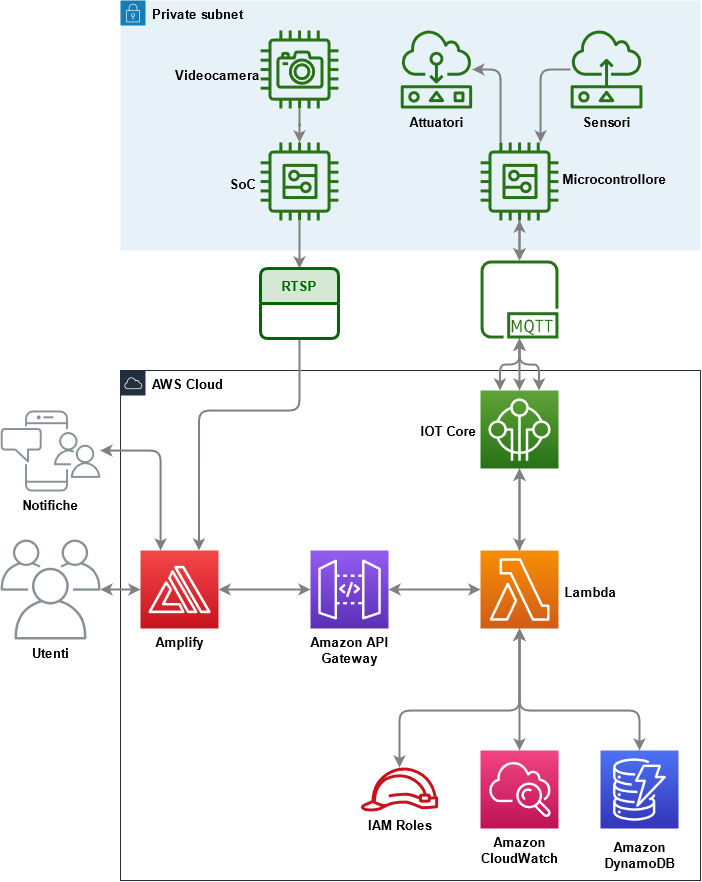
\includegraphics[width=0.8\textwidth]{DrawIo/Architecture.png}
    \end{figure}
    
    \section{Scelte Tecnologiche Cruciali}
        \subsection{AWS}
        Tra i servizi messi a disposizione da AWS vi è anche Amazon Cognito che permette di gestire gli utenti. 
        E' stato valutato Amazon Cognito ma è stato scartato perché gli utenti sono troppo pochi.
        
        \subsection{Protocolli di comunicazione}
        \subsubsection{Scambio messaggi}
        Come protocolli di comunicazione sono stati considerati i principali protocolli per la comunicazione IoT. Tra quelli di livello applicazione: 
        \begin{itemize}
            \item \textbf{AMQP (Advanced Message Queuing Protocol)}, protocollo che consente a un'ampia gamma di sistemi e applicazioni di interagire, creando messaggistica standardizzata su scala industriale.
            \item \textbf{CoAP (Constrained Application Protocol)}, protocollo adatto alle limitazioni di larghezza di banda e di rete, per dispositivi con capacità limitata, ma prevalentemente per la connessione nelle comunicazioni da computer a computer. 
            \item \textbf{DDS (Data Distribution Service)}, protocollo per comunicazioni peer-to-peer. In generale semplifica la distribuzione, incrementa l'affidabilità e riduce la complessità.
            \item \textbf{MQTT (Message Queue Telemetry Transport)}, protocollo di messaggistica progettato per comunicazioni IoT. MQTT usa un criterio di tipo publish-subscribe ed è ideale per dispositivi di dimensioni ridotte che richiedono efficienza a livello di larghezza di banda e uso della batteria.
        \end{itemize}
        La scelta è ricaduta su MQTT per la sua leggerezza ed efficienza, per la possibilità di instaurare comunicazioni bidirezionali tra molti dispositivi. Il design inoltre è molto semplificato dalla possibilità di creare topic a cui iscriversi o in cui pubblicare i messaggi.
        
        \subsubsection{Streaming Video}
        Per lo streaming video sono stati considerate due opzioni: streaming attraverso RTSP e attraverso HTTP con un server e HTML5. 
        RTSP è di sicuro la scelta più popolare perché adottato come protocollo dalle IP-cam e telecamere di sorveglianza. Nonostante ciò non è compatibile con HTTP e, non potendo fare lo stream su HTTP direttamente, non è visualizzabile nativamente dai browser. Questo protocollo è infatti usato internamente alle reti private. Volendo esporre il flusso video anche al di fuori della rete privata del committente la scelta è ricaduta sulla seconda opzione. Inoltre, con questa tecnologia alla videosorveglianza si ha accesso con qualsiasi browser, da computer o da smartphone.
        
        \subsection{Microcontrollori e Soc}
        \subsubsection{Hardware}
        Le piattaforme di sviluppo per l'IoT tenute presente sono state molteplici, da board con potenza computazionale più elevata, come Raspberry Pi, a scendere fino a ESP e le varianti Arduino. 
        
        Le board Arduino sono state scartate quasi subito, per la poca potenza computazionale e la necessità di moduli aggiuntivi per le connessioni. 
        La board RaspBerry Pi è stata scelta per task più computazionalmente onerosi, legati alla gestione ambientale, quali la video sorveglianza e l'analisi immagini. 
        Questa scelta non può essere invece adottata per la gestione delle gabbie. Le principali motivazioni risiedono nel fatto che il numero è variabile e il costo supererebbe molto superiore al budget. 
        La scelta in questo caso è ricaduta sull'ESP, non solo per il forte fattore cost-competitive, e per il supporto a Bluetooth e WiFi integrati, ma anche per il supporto della community e l'ottima potenza computazionale. Inoltre, rinunciando all'analisi immagini e alla qualità video a favore dei costi, il cliente potrà anche scegliere di sostituire la board Raspberry con un più economico ESP32-CAM.
        Con l'ESP8266 le prime settimane il lavoro di indagine preliminare ha rilevato qualche che risultava troppo limitato per utilizzare MicroPython.
        Tra ESP8266 e ESP32 è stato preferito quest'ultimo, anche per lasciare della capacità di calcolo per eventuali future espansioni e richieste del committente. 
        \subsubsection{Linguaggio di programmazione}
        Per quanto riguarda l'implementazione del codice nel microcontrollore, sono state presi in considerazione quattro scelte relative ai framework di sviluppo e ai linguaggi da adottare: 
        \begin{itemize}
            \item \textbf{C++} è il linguaggio attualmente più diffuso nell'ambito. 
            \item \textbf{Node-RED} è un tool di programmazione flow-based basato su browser, sviluppato su NodeJs e programmabile in JavaScript.
            \item \textbf{MicroPython} è un porting più leggero del compilatore Python3, eseguibile direttamente su microcontrollori. Include le principali librerie di Python e moduli aggiuntivi per l'accesso all'hardware di basso livello.
            \item \textbf{Espruino} è un interprete JavaScript open-source per microcontrollori. E' stato progettato per unità con poca RAM.
        \end{itemize}
        Sicuramente il più performante e con più librerie è C, ma risulta anche difficilmente testabile e pone challange non indifferenti per la configurazione dei sensori e per lo sviluppo di programmi molto complessi. Node-RED, basato su Node.js, ha il pieno vantaggio del suo modello non bloccante e event-driven. MicroPython d'altra parte offre un modello ad oggetti, testabile, sia semplice che elastico, con una buona base di librerie. Infine, Espruino, interprete JavaScript anch'esso, di facile utilizzo e dall'interfaccia semplificata. 
        I fattori chiave che il team ha preso in considerazione per la scelta sono stati: 
        \begin{itemize}
            \item la potenza espressiva rapportata alla chiarezza del linguaggio. 
            \item la testabilità del codice
            \item il numero di librerie e la futura possibilità di estensione del progetto.
        \end{itemize}
        Alla luce delle considerazioni fatte, si è scelto \textbf{MicroPython} per lo sviluppo, il testing e l'automatizzazione nei microcontrollori. Questo permette di allinearsi con l'utilizzo di \textbf{Pyhton} per il Raspberry.

    \section{Pattern Architetturali Utilizzati}
        \subsection{Client-Server}
        L'utilizzo del pattern client-server, nella videosorveglianza, ha permesso di esporre il flusso video su un server apposito e di accederci da qualunque dispositivo dotato di connessione. 
    
        \subsection{Pusblish-Subscribe}
        L'utilizzo del pattern publish-subscribe, è stata una scelta chiave per la modularità del sistema. La divisione in topic ha portato un maggiore ordine e una modellazione più vicina al vero dominio. 
        
        \subsection{Master-Slave}
        E' stato fatto uso dell'architettura master-slave per la gestione dei microcontrollori. Questa permette di espanderne il numero a piacimento, mandando istruzioni specifiche o generali per controllarne il comportamento.
        
        \subsection{Scheduling Cooperativo}
        Nei sistemi embedded è stato adottato lo scheduling cooperativo per evitare tante pitfall dello scheduling preemptive, quali l'interruzione di un processo di misura Real Time, quale quello della chiusura della valvola dell'acqua o la misura del battito cardiaco.
        
        \subsection{State Machine}
        Per definire il comportamento dei microcontrollori in maniera chiara è stata usata la modellazione con macchine a stati. Questa ha permesso di ridurre la probabilità di bug nel software e di isolare i componenti permettendo una futura espansione del comportamento. 
% -*- root: ../main.tex -*-
\chapter{Design di Dettaglio}

\section{Design Gestione Cibo e Acqua}
    Per l'automatizzazione e la gestione di cibo e acqua si è partiti dalle user-stories e dal modello del dominio costruito per sviluppare l'applicativo desiderato. Osservando i requisiti è stato progettato il modello fisico e l'interazione dell'animale con esso. 
    Si riporta di seguito il \textbf{design del prototipo fisico}, con i sensori e attuatori in giallo e la spiegazione del suo funzionamento [Fig. \ref{fig:ciboacqua}].
    Il design permette la modularità tra cibo e acqua, scegliendo all'occorrenza solo uno dei due o entrambi.
    \begin{figure}[H]
        \caption{Design Prototipo Cibo e Acqua (sensori e attuatori in giallo)}
        \label{fig:ciboacqua}
        \centering
        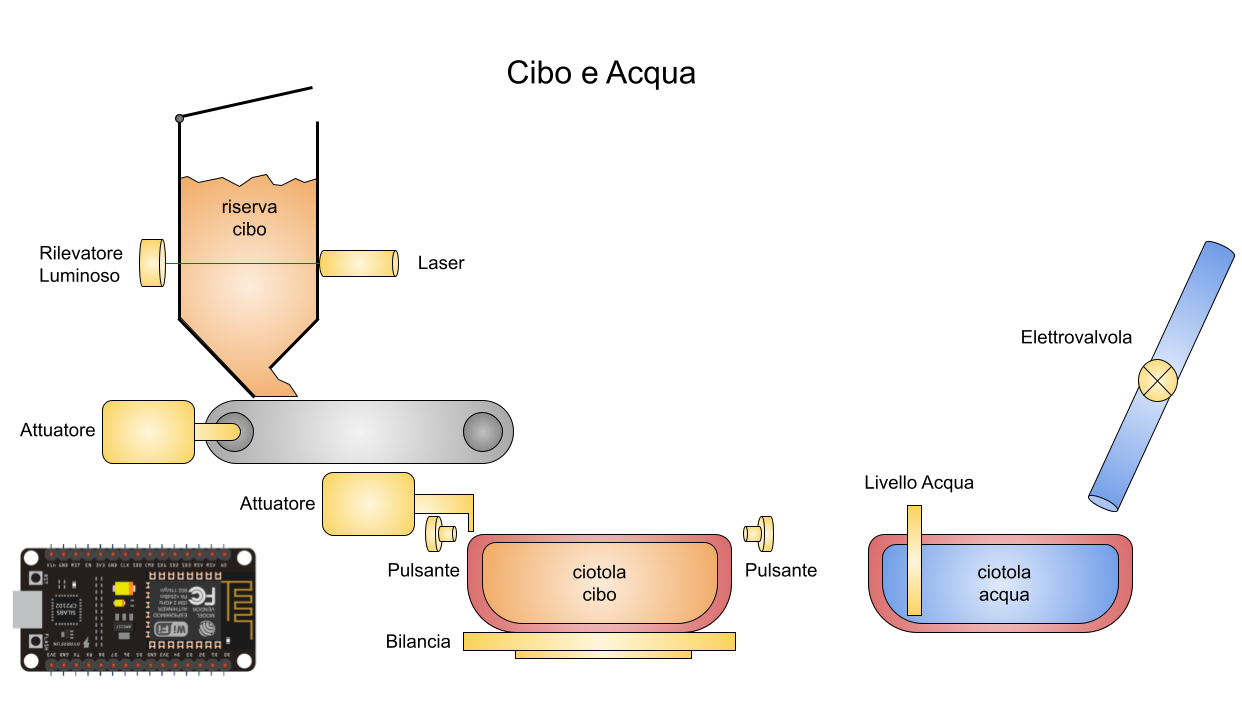
\includegraphics[width=1\textwidth]{Images/CiboAcqua.png}
    \end{figure}

    
    \subsection{Acqua}
    Per far fronte alla misurazione dei consumi, è stato innanzitutto necessario scegliere un sensore per ricavarne il \textbf{livello del liquido} [Fig. \ref{fig:ciboacqua}]. Il sensore deve ritornare un valore proporzionale alla percentuale di liquido rimanente. I consumi dell'animale a questo punto verranno inviati in cloud.
    
    Per quanto riguarda l'esigenza di riempimento dell'acqua, inizialmente la scelta era ricaduta su due sensori che rivelassero quando il liquido è al minimo o al massimo. In seguito questo design è stato semplificato usando direttamente il sensore introdotto per l'invio dei dati relativi al livello del liquido. 
    Successivamente è necessario che il sensore si interfacci con un'\textbf{elettrovalvola} [Fig. \ref{fig:ciboacqua}] per poter riempire la ciotola aprendo o chiudendo il flusso d'acqua all'occorrenza. 
    
    Il sistema deve essere modulare per design: qualora non si disponga del sistema idrico per poter rifornire la ciotola, devono comunque essere mandati i consumi con l'aggiunta di una notifica se se l'acqua sta per terminare.
    
    \subsubsection{Macchina a stati} Il comportamento è stato modellato come una macchina a stati [Fig. \ref{fig:statediagramWater}]. Ciò ha permesso di chiarire meglio le azioni del sistema a fronte di un avvenimento, il suo stato corrente e il suo comportamento generale.
    
    Inizialmente il comportamento prevede il controllo del \textbf{consumo di acqua}, ciclicamente e a intervalli regolari viene fatta una misurazione [Fig. \ref{fig:statediagramWater} "check water consumption"]. 
    
    E' stata stabilita una soglia minima di diminuzione del liquido per non incorrere in falsi positivi, dove le naturali oscillazioni del sensore potrebbero inviare consumi inesistenti. Talora questa soglia venisse superata, la \textbf{percentuale} di liquido consumata viene \textbf{inviata} in cloud, memorizzando l'ultima percentuale inviata [Fig. \ref{fig:statediagramWater} "send water consumption"]. Il sistema continua quindi a monitorare di nuovo il livello per ulteriori consumi. 
    
    Inevitabilmente il liquido nella ciotola andrà a finire, questo evento innescherà una transizione, dipendente dalla presenza o meno dell'elettrovalvola. 
    Se il sistema non prevede un rifornimento idrico il sistema passerà allo stato di \textbf{notifica di acqua esaurita} [Fig. \ref{fig:statediagramWater} "finished water notify"]. In questo stato una notifica verrà mandata all'addetto ai rifornimenti. Quando la ciotola verrà ricaricata il sistema passerà in automatico nuovamente allo stato per il controllo dei consumi.
    Qualora il sistema fosse dotato di elettrovalvola, la transizione innescata la aprirebbe, passando allo stato di \textbf{riempimento} [Fig. \ref{fig:statediagramWater} "fill water bowl"]. 
    
    In questo stato il livello viene controllato continuamente, per non incorrere in allagamenti indesiderati. 
    Un meccanismo di sicurezza temporizzato infatti controlla se un determinato periodo di tempo è passato senza che il sistema sia riuscito a riempire la ciotola con la valvola aperta. In caso affermativo il sistema va in blocco, chiudendo la valvola e passando allo stato di \textbf{notifica di errore} [Fig. \ref{fig:statediagramWater} "water system error notify"]. 
    Se il livello dell'acqua raggiunge il parametro desiderato invece lo stato torna a essere quello iniziale di osservazione.
    
    \begin{figure}[H]
        \caption{Macchina a Stati Acqua}
        \label{fig:statediagramWater}
        \centering
        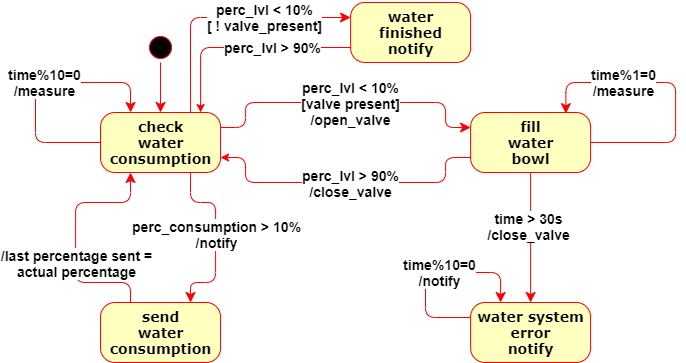
\includegraphics[width=1\textwidth]{DrawIo/stateDiagramWater.png}
    \end{figure}
    
    
    
    \subsection{Cibo}
    Per far fronte all'esigenza di monitorare i consumi di cibo dell'animale è stata introdotto un \textbf{sensore di peso} [Fig. \ref{fig:ciboacqua}]. Il sensore deve ritornare un valore proporzionale alla quantità di cibo presente nella ciotola. I consumi dell'animale verranno inviati in cloud. 
    
    Riguardo all'esigenza di rifornire il cibo, la bilancia si deve interfacciare con un attuatore che si occuperà della \textbf{distribuzione del materiale} [Fig. \ref{fig:ciboacqua} attuatore di sinistra]. Il design meccanico scelto è stato quello di un nastro trasportatore per la semplicità di realizzazione e l'efficacia. Altri design presi in esame comprendevano una botola che si aprisse e chiudesse, ma presentava problemi di forza per trattenere il cibo in caduta, e la vite di Archimede, ma presentava problemi nell'incastrarsi nel meccanismo dell'eventuale cibo in pezzi solidi. Il design con il nastro sfrutta la gravità per far cadere i pezzi su di esso e, all'attivazione, trascinarli con se permettendo ad altri di cadere. 
    La bilancia rileverà l'incremento e fermerà il sistema alla quantità desiderata.
    
    Per evitare che l'animale mangi il cibo durante la distribuzione, falsandone le misure, è stato introdotto un altro \textbf{attuatore bidirezionale} [Fig. \ref{fig:ciboacqua}] per estendere o ritrarre uno sportellino che ne previene l'accesso.
    Per determinare quando lo sportellino arriva al massimo o al minimo della sua estensione sono stati introdotti \textbf{due pulsanti} [Fig. \ref{fig:ciboacqua}] che segnalano quando fermare il movimento. 
    
    Infine per segnalare quando il cibo di scorta sta anch'esso per finire sono stati introdotti un \textbf{laser e un sensore luminoso} [Fig. \ref{fig:ciboacqua}] nella riserva di cibo. Se il cibo è presente il fascio laser verrà interrotto e il sensore non rileverà alcuna luce. Quando il cibo durante l'erogazione scende sotto una soglia critica, il fascio raggiunge il dispositivo di sensing e una notifica verrà inviata all'addetto. 
    
    Anche qui il sistema deve essere modulare per design: qualora non ci si voglia avvalere del sistema per rifornire la ciotola, i consumi devono comunque essere mandati in cloud con l'aggiunta di una notifica se il cibo nella ciotola sta per terminare.
    
    \subsubsection{Macchina a stati} Anche in questo caso il comportamento, data la sua complessità, è stato modellato come una \textbf{macchina a stati} [Fig. \ref{fig:statediagramFood}]. Il comportamento è simile alla macchina a stati mostrata in precedenza, essendo l'attuatore per il rifornimento del cibo paragonabile all'elettrovalvola e la bilancia paragonabile al sensore di livello dell'acqua. 
    
    Inizialmente il comportamento prevede il \textbf{controllo dei consumi} in maniera ciclica tramite la bilancia [Fig. \ref{fig:statediagramFood} "check food consumption"].
    Anche in questo caso talora la soglia minima venisse superata, la \textbf{quantità consumata viene inviata} in cloud [Fig. \ref{fig:statediagramFood} "send food consumption"]. Il sistema continua quindi a monitorare di nuovo il peso per ulteriori consumi.
    
    Se è stato scelto di non usufruire della parte di rifornimento cibo, il sistema quando questo si verrà ad esaurire, passerà allo \textbf{stato di notifica} [Fig. \ref{fig:statediagramFood} "food finished notify"]. Similmente al comportamento del sistema per l'acqua , quando la ciotola verrà ricaricata il sistema passerà in automatico nuovamente allo stato per il controllo dei consumi.
    In caso fosse presente il sistema di ricarica cibo completo, l'attuatore per chiudere l'accesso al cibo si attiverà, passando allo \textbf{stato di chiusura} [Fig. \ref{fig:statediagramFood} "blocking food access"]. Una volta completata la chiusura il nastro per l'erogazione del cibo verrà attivato e il sistema passerà allo \textbf{stato di erogazione} [Fig. \ref{fig:statediagramFood} "fill food bowl"]. Se non fosse presente lo sportellino per l'accesso al cibo, dallo stato iniziale si passerà direttamente a quest'ultimo attivando il nastro, senza il passaggio intermedio. 
    
    In questo stato il livello viene controllato continuamente, per un dosaggio corretto. Assieme al peso del cibo erogato, viene controllata anche la presenza del fascio laser. Qualora venisse rilevato significa che il cibo di scorta sta per finire e una notifica viene inviata all'addetto.
    Anche in questo caso è presente un meccanismo di sicurezza temporizzato che, dopo un periodo di tempo massimo, blocca l'erogazione e \textbf{passa allo stato di notifica errore} di sistema [Fig. \ref{fig:statediagramFood} "food system error notify"]
    
    In caso il cibo invece raggiunga la quantità desiderata, il sistema tornerà allo stato iniziale, garantendo eventualmente l'accesso al cibo tramite lo \textbf{stato di apertura} [Fig. \ref{fig:statediagramFood} "allowing food access"]    
    
    \begin{figure}[H]
        \caption{Macchina a Stati Cibo}
        \label{fig:statediagramFood}
        \centering
        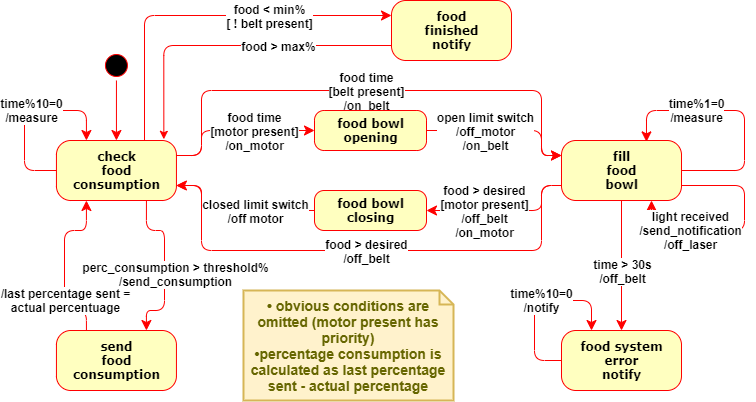
\includegraphics[width=1\textwidth]{DrawIo/stateDiagramFood.png}
    \end{figure}
    
    
\section{Design Monitoraggio Parametri Vitali}
Per il monitoraggio dei parametri vitali il design fisico è stato semplificato di molto, richiedendo due sensori e un microcontrollore. Il \textbf{design del prototipo fisico}, con i sensori in giallo e la spiegazione del suo funzionamento [Fig. \ref{fig:collare}] sono riportati di seguito.
    \begin{figure}[H]
        \caption{Design Prototipo Collare}
        \label{fig:collare}
        \centering
        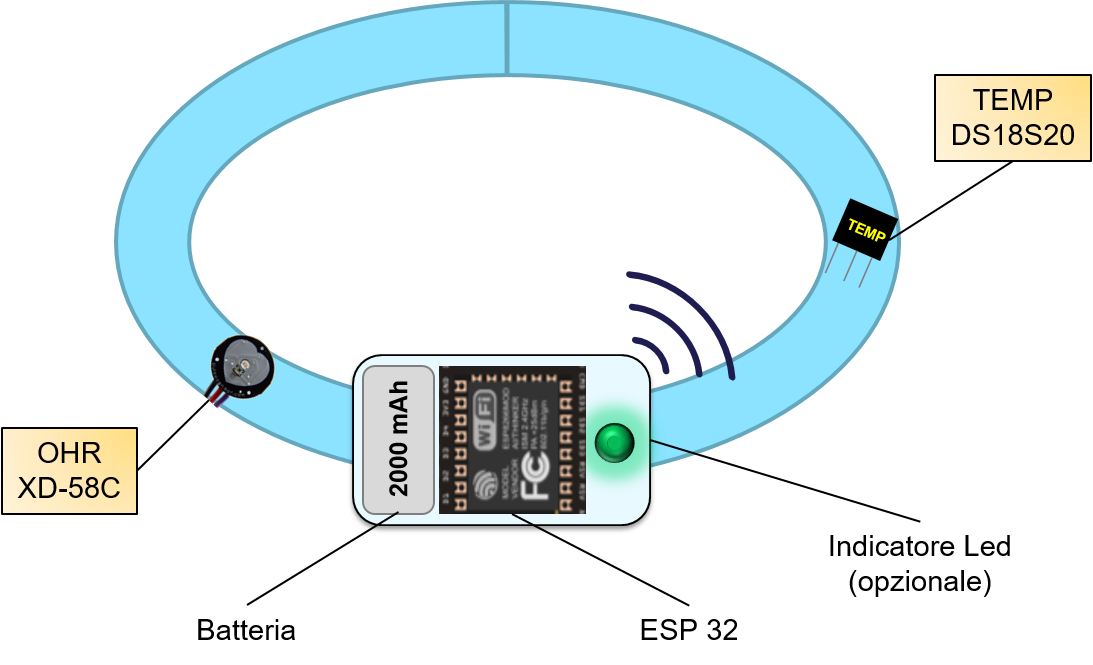
\includegraphics[width=1\textwidth]{Images/collare.png}
    \end{figure}
Il primo device di sensing necessario è quello di \textbf{temperatura}, che periodicamente deve inviare i valori letti al cloud. Eventualmente, se i valori sono fuori norma, deve segnalarlo inviando una notifica immediatamente.
Il secondo sensore è necessariamente quello dei \textbf{battiti}. Anch'esso deve inviare a intervalli regolari i battiti per minuto in cloud, affinché vengano registrati. Opzionalmente sarà presente un LED per visualizzare i battiti in real-time. In caso di anomalie tali da portare i valori oltre il minimo o il massimo, una notifica deve essere mandata tempestivamente. 
La macchina a stati si compone semplicemente di due stati divisi che ciclano su loro stessi, inviando periodicamente i valori letti ed eventualmente le notifiche per le anomalie.
    
\section{Design Videosorveglianza}
Per la videosorveglianza il design ha richiesto necessariamente, come descritto in precedenza, una board più potente che sostenesse l'elaborazione delle immagini. Di seguito il \textbf{design del prototipo fisico}, con i sensori in giallo e la spiegazione del suo funzionamento [Fig. \ref{fig:canile}]. 
    \begin{figure}[H]
        \caption{Design Prototipo Monitoraggio Canile (sensori in giallo)}
        \label{fig:canile}
        \centering
        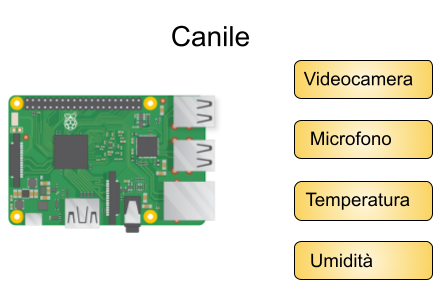
\includegraphics[width=0.6\textwidth]{Images/Canile.png}
    \end{figure}
Per quanto riguarda i sensori, ovviamente è necessaria una \textbf{videocamera}, che catturi l'ambiente circostante e mandi il flusso video alla board per un analisi. Oltre alla videocamera, opzionalmente, sono stati modellati un \textbf{sensore di temperatura e umidità}, per salvare in cloud i parametri ambientali del canile, e un \textbf{device di sensing sonoro}, per rilevare suoni forti continuativi.
La board deve anche fornire opzionalmente lo streaming video della telecamera, facendo da server, per l'addetto alla sorveglianza. 
Il flusso dei dati è chiaramente unidirezionale, dai sensori e dalla webcam verso l'esterno, come da architettura generale [Fig. \ref{fig:DesignArchitettura}].

\section{Design del Database}
Per immagazzinare i dati necessari all'applicazione si è deciso di utilizzare \textbf{Dynamo DB}.
Il database principale doveva immagazzinare:
\begin{itemize}
    \item I \textbf{profili} dei \textbf{cani} presenti all'interno del canile;
    \item Gli \textbf{orari} e le \textbf{quantità} di cibo da somministrare a seconda del cane;
    \item I \textbf{valori} rilevati dai dispositivi di \textbf{sensing}, che comprendono:
    \begin{itemize}
        \item Temperatura corporea;
        \item Frequenza cardiaca;
        \item Consumo di acqua; 
        \item Consumo di cibo;
        \item Temperatura ambientale del canile;
        \item Umidità rilevata all'interno del canile;
    \end{itemize}
    \item I profili degli \textbf{utenti}.
\end{itemize}

La progettazione del database è stata portata a termine seguendo diversi passaggi:
    \begin{enumerate}
        \item Definizione di uno schema \textbf{ER} da utilizzare come base di partenza;
        \item Individuazione degli \textbf{accessi} mediante la definizione delle \textbf{query} principali;
        \item Definizione dei \textbf{pattern} di Primary Key e Sort Key;
        \item Introduzione di indici e campi aggiuntivi;
    \end{enumerate}
    
    \subsection{Definizione di un ER}
    Nonostante non si tratti di un database relazionale, abbozzare uno schema Entity Relationship può essere utile per avere una buona visione di partenza di come devono essere gestiti i dati.
    \subsubsection{Informazioni sui cani}
    Il primo schema ad essere stato elaborato è stato quello che racchiude tutto ciò che ha a che fare con i dati di un cane, ovvero il profilo del cane, i dettagli della sua relativa distribuzione del cibo e le rilevazioni di cibo, acqua, temperatura e battiti che lo riguardano.
     \begin{figure}[H]
        \caption{ER dati del cane}
        \label{fig:dogER}
        \centering
        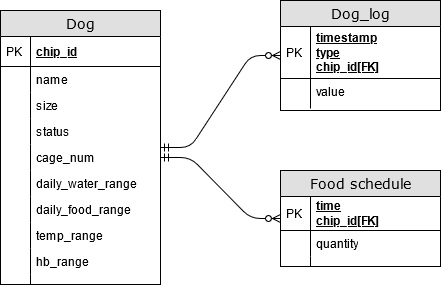
\includegraphics[width=0.6\textwidth]{DrawIo/EntityRelationship.png}
    \end{figure}
    \begin{itemize}
            \item \textbf{Cane}: il profilo del cane è modellato mediante la tabella \texttt{Dog} che, oltre alle consuete informazioni presenta anche le soglie, impostate dal veterinario, al di fuori delle quali si rileva un'anomalia.   
            
            \item \textbf{Programma dei pasti}: l'entità \texttt{Food\_Schedule} immagazzina gli orari e le quantità dei pasti. Il criterio secondo cui, nel caso standard, vengono decisi questi dati è la taglia, tuttavia si è deciso di collegare l'entità direttamente al cane poiché ciò permette di effettuare una programmazione più a grana fine. In questo modo, infatti, si può consentire ad un veterinario di effettuare modifiche sul regime alimentare di un unico cane, senza influenzare gli altri cani della stessa taglia.
            
            \item \textbf{Rilevazioni}: nello schema in figura è già stata collassata la gerarchia delle rilevazioni sopra elencate, concentrandole nell'entità \texttt{Dog\_log} che ne distingue la natura mediante il campo \texttt{type}.
       \end{itemize}
     \subsubsection{Informazioni sugli utenti}
     In fase di progettazione si voleva che il database gestisse anche gli utenti che agiscono sul sito, in maniera tale che ne fossero definiti i ruoli in base ai quali avrebbero avuto diversi permessi e una diversa visualizzazione dei dati sul sito web.
     Questo ER si distacca da quello relativo ai cani e si presenta in questo modo:
         \begin{figure}[H]
        \caption{ER utenti}
        \label{fig:userER}
        \centering
        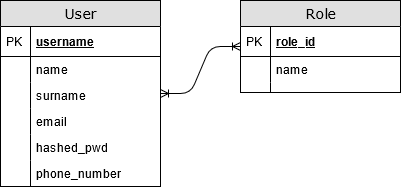
\includegraphics[width=0.6\textwidth]{DrawIo/UserER.png}
    \end{figure}
    
    \subsubsection{Rilevazioni ambientali}
    Anche per quanto riguarda le rilevazioni ambientali ci si trova di fronte a un'area separata dalle precedenti, perché non ha alcun tipo di correlazione né con i cani, né con gli utenti. Esse sono modellate con una tabella di nome \texttt{Env\_Logs} che ne immagazzina il \texttt{timestamp}, il \texttt{type}, che serve a distinguere le rilevazioni di temperatura e quelle di umidità e il \texttt{value} che, nel caso della temperatura è espresso in gradi mentre nel caso dell'umidità è espresso in percentuale. 

    \subsection{Individuazione degli accessi}
    Una volta ottenuta una bozza dello schema Entity Relationship si è passati a definire gli accessi in base alle query che sarà necessario chiamare per interrogare il database.
    Definire gli accessi si rivela essere di vitale importanza quando si lavora con un database come DynamoDB perché permette di impostare le tabelle in modo da rendere più facile l'accesso ai dati più richiesti. Per permettere ciò si è portati anche a introdurre delle ridondanze e a sacrificare l'integrità referenziale prediligendo i benefici sulle performance.
    Di seguito le interrogazioni suddivise per frequenza
    \begin{itemize}
    \item \textbf{Frequenza molto elevata} (ogni pochi minuti)
            \begin{itemize}
                \item inserimento di una rilevazione riguardante consumi, parametri vitali del cane, valori ambientali
            \end{itemize}
    \item \textbf{Frequenza elevata} (poche volte all'ora)
            \begin{itemize}
                \item visualizzazione dei cani presenti
                \item visualizzazione dei consumi di un cane
                \item visualizzazione dell'ultima rilevazione di temperatura e battiti di un cane
            \end{itemize}
    \item \textbf{Frequenza media} (una o poche volte al giorno)        
            \begin{itemize}
                \item visualizzazione storico delle rilevazioni di un cane
                \item visualizzazione dei consumi di un cane
                \item inserimento di un nuovo cane 
                \item interrogazione sull'orario e la quantità dei pasti
                \item a fine giornata, comparazione dei consumi totali di acqua e cibo odierni, per ciascun cane, con i rispettivi range giornalieri contenuti nel profilo dell'animale.
            \end{itemize}
    \item \textbf{Frequenza bassa} (meno di una volta a settimana)        
        \begin{itemize}
            \item impostazione delle soglie dei consumi di un cane oltre le quali vi è un'anomalia
            \item impostazione delle soglie dei parametri vitali di un cane oltre le quali vi è un'anomalia
            \item aggiornamento del programma dei pasti
            \item aggiornamento dello stato di un cane 
        \end{itemize}
    \end{itemize}
    
    \subsection{Definizione dei pattern di Primary Key e Sort Key}
    Dopo aver individuato le interrogazioni che verranno fatte sul database e le loro frequenze si è passati alla progettazione vera e propria dell'\textbf{unica tabella} del database. A differenza di un database relazionale, infatti, DynamoDB non permette di ricorrere alle \textbf{join}, se non con dei workaround la quale adozione è un chiaro sintomo del fatto che non si è scelta correttamente la tipologia di database da adottare. 
    La tabella che è stata creata è strutturata con i seguenti campi:
\begin{itemize}
    \item \textbf{PK}: o Primary Key, è la chiave primaria e consiste in una stringa che determinerà la natura del record a cui appartiene. 
    \item \textbf{SK}: o Sort Key, è la chiave di ordinamento e consiste anch'essa in una stringa che segue uno specifico pattern e che assieme alla PK determinerà univocamente il record.
    \item \textbf{Altri campi}: che sono dati dall'unione dei campi di tutte le entità che si è deciso di coinvolgere, con l'aggiunta di alcuni campi introdotti per fornire un'indicizzazione o per inserire delle ridondanze che facilitino l'accesso.
    
    I pattern che sono stati definiti per PK e SK sono i seguenti:
        \begin{figure}[H]
        \caption{Pattern PK e SK suddivisi per entità di riferimento}
        \label{fig:KeyPattern}
        \centering
        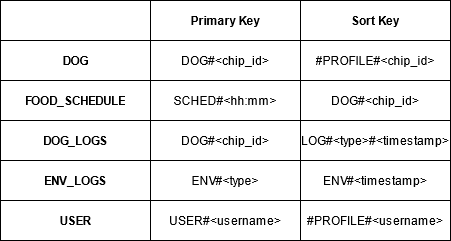
\includegraphics[width=0.6\textwidth]{DrawIo/KeysPattern.png}
    \end{figure}
\end{itemize}
    Dalla tabella, oltre ai pattern per i valori delle chiavi è possibile anche intuire il modo in cui si è deciso di effettuare la trasposizione dallo schema relazionale. Si può notare infatti che:
    \begin{itemize}
        \item \textbf{\texttt{Food\_Schedule}}: si è deciso di mantenere la programmazione dei pasti separata dai dati del cane poiché mantenerla come struttura dati all'interno del profilo avrebbe reso meno immediata la modifica e il recupero degli orari e delle quantità che il sistema automatizzato deve erogare.  
        \item \textbf{\texttt{Dog\_Log}}: la stessa decisione è stata presa per quanto riguarda i dati delle rilevazioni, poiché la query che permette l'inserimento di questi dati è quella che verrà chiamata con la massima frequenza ed era quindi importante facilitarne la fruizione.
        \item \texttt{\texttt{User}}: una sorte diversa è spettata ai ruoli ricoperti dagli utenti. Si è deciso di modellare i ruoli come una set di stringhe all'interno del profilo dell'utente, poiché si tratterebbe di un campo che viene modificato raramente.
    \end{itemize}
    
    \subsection{Introduzione di indici e campi aggiuntivi}
    L'ultima fase è stata quella di individuare quali altre modifiche potevano essere apportate al risultato finale della tabella per favorire le interrogazioni.
    Si è deciso pertanto di:
    \begin{itemize}
        \item aggiungere i \textbf{campi} \texttt{last\_temp} e \texttt{last\_hb} nel profilo del cane per permettere una più prestante interrogazione nel momento in cui, nella homepage del sito si vogliono visualizzare le ultime rilevazioni dei parametri vitali del cane. In assenza di questi due campi sarebbe stato necessario interrogare il database con un range di timestamp sensato per ottenere una fetta dello storico delle rilevazioni, ordinarle e restituire la più recente. Questo per la temperatura che per la frequenza cardiaca.
        \item aggiungere un nuovo \textbf{indice} sul campo \textbf{\texttt{size}} per permettere di effettuare alcune query basandosi sulla taglia del cane.
    \end{itemize}
    
    
\section{Design WebApp}

La WebApp è stata suddivisa in due \textbf{Macro} aree:
\begin{itemize}
    \item \textbf{Login}: la schermata si occupa di fornire un accesso base all'utente, l'unica funzione esposta è la possibilità di effettuare il \textbf{login}, attualmente rappresenta un placeholder, dato che non contine alcuna logica né funzione utile, questo per concentrarsi maggiormente su aspetti più inerenti. 
    \item \textbf{Home}: fornisce tutte le funzioni principali dell'applicativo,
    la schermata è divisa in schede, ogni scheda è a sua volta divisa in più componenti, uno per la visualizzazione dei cani presenti e uno per le azioni specifiche da attuare su di esso, o in generale.
    L'unica scheda che contiene un solo
    
    dove ogni scheda consente determinate operazioni:
    \begin{itemize}
        \item \textbf{Gestore}: Consente di effettuare le principali azioni del sito, inoltre può anche effettuare le azioni seguenti.
        \item \textbf{Addetto alla salute}: Può visualizzare i parametri vitali e lo stato di salute degli animali.
        \item \textbf{Addetto ai rifornimenti}: Può visualizzare i dati di un cane, i suoi consumi e impostare l'orario e la quantità di cibo.
        \item \textbf{Addetto alla sorveglianza}: Puù visualizzare lo streaming video.
        \item \textbf{Altro addetto}: placeholder per funzioni future
    \end{itemize}    
    
\end{itemize}


\section{Design Serverless Application}

L'esposizione delle funzioni del back-end, segue a braccetto la definizione delle query necessarie per interrogare e inserire nuovi dati all'interno di DynamoDB.

Le funzioni sono state divise per innesco, dove abbiamo: 
\begin{itemize}
    \item Lambda ad innesco \textbf{API REST}: rappresentano la maggioranza delle funzioni, sono ulteriormente divise in base allo scopo di interrogazione(GET) o inserimento(POST)
    \item Lambda ad innesco \textbf{Crono}: i consumi dei cani sono controllati a fine giornata per verificare che le soglie dei consumi siano nei parametri. 
    l'innesco avviene tramite eventi \textbf{CloudWatch}
    \item Lambda ad innesco \textbf{MQTT}: rappresentano i diretti inserimenti delle rilevazioni all'interno del database, sono in ascolto su un sul topic \textbf{ESP/\#}, questo consente di ascoltare tutti i messaggi provenienti da i sotto topic.
\end{itemize}



% -*- root: ../main.tex -*-

% Esporre i principali problemi affrontati durante l'effettiva realizzazione delle componenti hardware/software e illustrare le soluzioni implementative adottate. Se l'elaborato ha previsto l'utilizzo di tecnologie già disponibili sul mercato, discuterne brevemente le caratteristiche e motivarne l'adozione rispetto ad altre soluzioni assimilabili. NOTA: in questa sezione devono essere riportate esclusivamente le porzioni di codice ritenute particolarmente significative.
% 10000 - 21000 battute

\chapter{Implementazione}
\section{Microcontrollori}
\subsection{Battito Cardiaco}
Un parte particolarmente complessa è stata quella della modellazione del sensore per il battito. Il sensore, qualora interpellato, fornisce un singolo valore direttamente proporzionale alla dilatazione dei vasi sanguigni. Ne deriva la necessità di attuare misurazioni frequenti per non incorrere nella perdita della breve variazione di un battito. Abbiamo stabilito la frequenza di campionamento in base a quanto segue:
Considerando che in condizioni di riposo, i battiti per minuto di un cane - da intendersi come pulsazioni - sono generalmente compresi tra 60 e 140 bpm, in base alla taglia, età e razza, e il valore può raggiungere valori anche più alti qualora in movimento, abbiamo preso come valore limite da rilevare 150 bpm. Ciò, significa che il tempo di ogni ciclo cardiaco $T_{cc}$ è:
\begin{equation}
T_{cc} = \frac{1}{bps} = \frac{1}{\frac{bpm}{60}}= \frac{60}{bpm} \Rightarrow \frac{60}{150 bpm} = 0.4s
\end{equation}
Considerato che il ciclo cardiaco si compone in sistole (contrazione) e diastole (rilassamento), la fase sistolica è quella più facilmente rilevabile poiché la contrazione ventricolare causata è più violenta e breve. Questa fase durante le rilevazioni effettuate dura circa un mezzo del ciclo cardiaco e produce un picco nei valori particolarmente indicativo per rilevare il battito in mezzo al naturale rumore del sensore. Per non perdere il picco massimo il numero di campionamenti $N_{c}$ durante questa fase è stato fissato a 20. La frequenza di campionamento minima risultante $f_{min}$ è stata calcolata come: 
\begin{equation}
f_{min} = \frac{ \frac{1}{2} *  T_{cc} }{N_{c}} \Rightarrow  \frac{ \frac{1}{2} *  0.4s }{20} = 0.01s = 10 ms 
\end{equation}

Salvando i valori risultanti e graficandoli con la libreria python "Mathplotlib" si ottiene una linea come quella di colore rosso in [Fig. \ref{fig:Heartbeat}]. Si può notare che il campionamento è sufficiente e permette di distinguere intuitivamente i battiti. 
Per rilevare le pulsazioni a livello digitale però è necessario formalizzare un altro modello matematico che non faccia incorrere il sistema in falsi positivi o falsi negativi. Un primo approccio si è basato su stabilire una singola soglia, oltre la quale il battito è rilevato e registrato. Questa soluzione si è rivelata inadatta in quanto il disturbo del sensore la farebbe attraversare più volte (si veda in [Fig. \ref{fig:Heartbeat}] poco prima del campionamento numero 2400 il valore attraversa la linea azzurra parecchie volte). Inadatti si sono rivelati anche i tentativi di normalizzare la linea dei valori, in quanto parecchio discontinui e di frequenza elevata, si perde la differenziazione dei picchi. Si è optato per stabilire una doppia soglia, la prima, più alta, oltre la quale il battito è rilevato, la seconda, più bassa, che determina la fine del battito. La prima volta che il valore attraversa la prima [Fig. \ref{fig:Heartbeat}, linea azzurra] una variabile registra il battito e nessun altra registrazione viene effettuata sino a che i valori non scendono sotto la soglia di fine battito [Fig. \ref{fig:Heartbeat}, linea gialla]. 
Queste soglie non possono essere fisse, variando la pressione di animale in animale e pure di giorno in giorno per lo stesso essere vivente. Per questo motivo i valori sono stati fissati per la prima a 4/5 e per la seconda a 1/2 tra minimo [Fig. \ref{fig:Heartbeat}, linea verde] e massimo [Fig. \ref{fig:Heartbeat}, linea blu] dei precedenti valori. La grandezza della finestra dei valori da cui prendere minimo  e massimo è stata fissata a 250 valori. Questo perché, come si può notare dal grafico, comprende almeno due battiti. Un range troppo piccolo creerebbe dei minimi e massimi locali, rilevando picchi non propri e dando parecchi falsi positivi. Una finestra troppo ampia porterebbe a una staticità delle soglie rispetto alla variazione di pressione che creerebbe falsi negativi.  

    %GRAFICO BATTITO
    \begin{figure}[H]
        \caption{Grafico Battiti}
        \label{fig:Heartbeat}
        \centering
        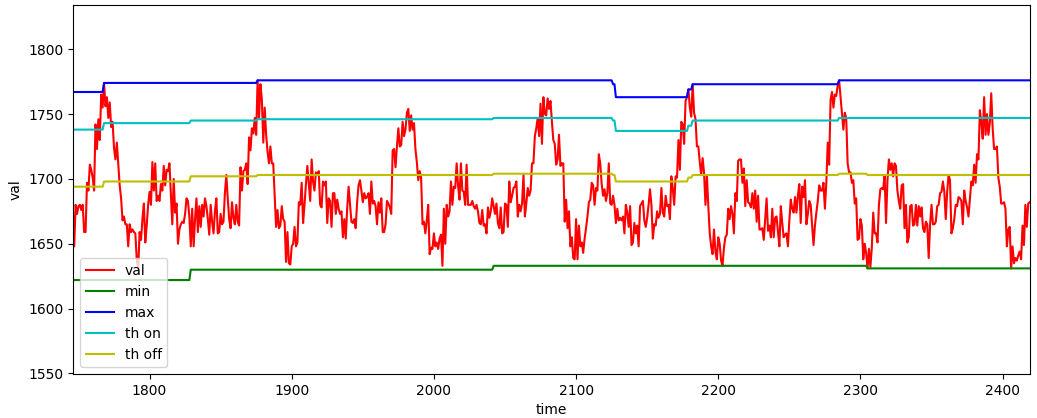
\includegraphics[width=1\textwidth]{Images/heartbeatGraph.png}
    \end{figure}

Una volta rilevati i singoli battiti con il modello matematico, il calcolo del battiti al minuto è stato realizzato salvando la cronologia degli istanti di tempo per gli ultimi N battiti $N_{beats}$. Sperimentalmente si è optato per 30 registrazioni per mantenere il valore dei bpm reattivo ma non dipendente solo da poche unità. Prelevando dalla cronologia il tempo passato $T_{diff}$ per questi battiti, si può facilmente derivare il rateo di $bpm$ attuale tramite la formula: 
\begin{equation}
bpm = \frac{ N_{beats}*60 s/min }{T_{diff}} = \frac{ N_{beats}*60 s/min }{T_{last}-T_{first}} 
\end{equation}
Il battito cardiaco risultante viene poi inviato periodicamente al Database e, qualora ci fossero anomalie, una notifica viene invece generata e inviata immediatamente.
\begin{tcolorbox}[tab2,tabularx={c||c|c|Y|Y},title=Confronto Prestazioni Microcontrollori Testati,boxrule=0.5pt] \hline
board & velocità processore & costo & tempo medio avvio programma & tempo medio connessione MQTT \\ \hline
\hyperlink{https://en.wikipedia.org/wiki/ESP8266}{ESP8266} & 160 MHz & 5€ & 8,1 s & 9,3 s\\ \hline
\hyperlink{https://en.wikipedia.org/wiki/ESP32}{ESP32} & 240 MHz (dual core) & 7€ & 5,2 s & 3,4 s\\ \hline
\end{tcolorbox}

\input{Tex/Implementation/SaraKiade}
\input{Tex/Implementation/GyordanCaminati}

% -*- root: ../main.tex -*-
\chapter{Iterazioni}
Gli sprint sono stati portati avanti nel seguente modo:
    \paragraph{Sprint Planning}
        Pianificazione a inizio sprint degli obiettivi, tempistiche e responsabilità nel periodo dello sprint corrente. Diviso in due parti:
        \begin{itemize}
        \item\textbf{parte 1} 
            Viene raffinato e rivisto il product backlog, viene effettuata la scelta dello sprint goal (what).
        \item\textbf{parte 2}
            Si decidono gli item e viene raffinato come implementarli (how). Effettuato con solo il team senza la figura del product owner
        \end{itemize}
    \paragraph{[Iterativo] Daily scrum} Breve meeting svolto giornalmente. Viene utilizzato per gli aggiornamenti sull'andamento del progetto, senza scendere nei dettagli implementativi.
    \paragraph{[Occasionale] Pair Programming } Utilizzato per risolvere problemi che causano il blocco di un componente del team per parecchio tempo su una issue.
    \paragraph{Meeting finale}
        Riflessioni e considerazioni finali sullo spint passato. Suggerimenti per migliorare il prossimo. Diviso in tre parti: 
        \begin{itemize}
        \item\textbf{Product backlog refinement} aggiunta di dettagli e riordino del product backlog
        \item\textbf{Sprint review} è stato ispezionato l'incremento, il Minimum Viable Product o di risultati sul processo. Discernere cosa è stato fatto e cosa no
        \item\textbf{Retrospettiva} Considerazioni sul team stesso e sui miglioramenti per il prossimo sprint. 
        \end{itemize}

\section{Sprint 0}
All'interno dello sprint 0 il focus è stato sullo scegliere le giuste tecnologie di sviluppo e sull'apprenderle in maniera sufficiente per il kick-off del progetto.
L'obiettivo è stato raggiungere una conoscenza e competenza minima per sviluppare il design in maniera consapevole e ottimale.
\paragraph{Deliverables} 
al termine di questo sprint si sono acquisite le competenze di base per poter iniziare a lavorare con AWS e i dispositivi IoT. Inoltre ci si è portati avanti con lo scheletro del sito.
\begin{itemize}
    \item ambiente di lavoro Linux standardizzato e virtualizzato
    \item sito linkato, con le prime due pagine base: home e login
    \item ESP32 con firmware installato MicroPython, script e guida all'uso
    \item codice per sensori base, test relativi e stubs per eseguirli senza necessità del micro-controllore
    \item repository software con CI e test automatizzati 
    \item database progettato e popolato con qualche dato ai fini di testing
\end{itemize}

\section{Sprint 1}
All'interno dello sprint 1 il focus è stato sull'usare le competenze tecnologiche acquisite precedentemente per sviluppare i componenti principali del progetto. Sono stati scelti come obiettivi le user stories per l'automatizzazione di cibo e acqua e la visualizzazione delle informazioni relative a un animale sulla webpage.
\paragraph{Deliverables}
al termine di questo sprint sono state implementate le funzioni base dei maggiori componenti per l'automatizzazione fisica di cibo e acqua e il relativo prototipo fisico. Sono state aggiunte sull'applicativo la vista delle informazioni dell'animale e l'impostazione del cibo da erogargli. 
\begin{itemize}
    \item codice per i sensori/attuatori per acqua e cibo, con stubs, test e automatizzazione. (Livello acqua, elettrovalvola, motore, bilancia, laser e rilevatore di luce)
    \item prototipo fisico per i sensori per acqua e cibo. 
    \item database migliorato e rifattorizzato
    \item visualizzazione dei dati del cane sul sito 
    \item visualizzazione dei grafici delle statistiche sul sito 
\end{itemize}

\section{Sprint 2}


\section{Sprint 3}


\section{Sprint 4}



% -*- root: ../main.tex -*-
\chapter{Conclusioni}

\nocite{*} % Includes all references from the `references.bib` file
\printbibliography[title={Bibliografia completa}]

\end{document}
